\documentclass[12pt]{report}
\usepackage{graphicx}
\usepackage[utf8]{inputenc}
\usepackage{hyperref}
\usepackage[T1]{fontenc}
\usepackage{titlesec}
\usepackage{lmodern}
\usepackage[french]{babel}
\usepackage[acronym]{glossaries}
\usepackage{amsmath}              % pour les formules mathématiques          % 
\usepackage{cite}  
\usepackage{float}



\usepackage{url}
\usepackage[a4paper, left=2.5cm, right=2.5cm, top=1.8cm, bottom=1.8cm]{geometry}

\makeglossaries
\newglossaryentry{fasttext}{
    name=FastText,
    description={Modèle développé par Facebook AI pour des représentations vectorielles de mots prenant en compte les sous-mots}
}

\newacronym{tln}{TALN}{Traitement Automatique du Langage Naturel}
\newacronym{ia}{IA}{Intelligence Artificielle}
\newacronym{rnn}{RNN}{Réseau de Neurones Récurrents}
\newacronym{lstm}{LSTM}{Long Short-Term Memory}
\newacronym{gru}{GRU}{Gated Recurrent Unit}
\newacronym{pubmedbert}{PubMedBERT}{PubMed BERT, un modèle de langage préentraîné spécifique au domaine biomédical}
\newacronym{biobert}{BioBERT}{BioBERT, une variante de BERT pour le domaine biomédical}
\newacronym{smote}{SMOTE}{\textit{Synthetic Minority Over-sampling Technique} (technique de suréchantillonnage synthétique pour les classes minoritaires)}
\newacronym{bert}{BERT}{Représentations encodées bidirectionnelles des transformeurs}
\newacronym{glove}{GloVe}{Vecteurs globaux pour la représentation de mots}
\newacronym{w2v}{Word2Vec}{méthode d'apprentissage de représentations vectorielles des mots développée par Mikolov et al.}
\newacronym{fsl}{FSL}{Few-Shot Learning}
\newacronym{auc}{AUC}{Area Under the Curve}
\newacronym{cnn}{CNN}{Convolutional Neural Networks}
\newacronym{tsne}{t-SNE}{Projection Stochastique Voisine en Faible Dimension (\textit{t-distributed Stochastic Neighbor Embedding})}


\begin{document}
\sloppy

\begin{titlepage}
    \begin{center}
        
\includegraphics[width=7cm]{images/uliege.jpg} \\[1cm]
        
        {\Huge \textsc{Université de Liège}} \\[0.5cm]
        {\Large Faculté des Sciences Appliquées} \\[2.5cm]
        
        \rule{\linewidth}{0.8mm} \\[0.4cm]
        
        {\LARGE \textbf{Classification de textes biomédicaux à l’aide de  LSTM, GRU et de l’attention de \\ Bahdanau}} \\[0.4cm]
        
        \rule{\linewidth}{0.8mm} \\[1cm]
        
        {\large 
         Mémoire présenté en vue de l’obtention du diplôme de \\[0.3cm]
        \textit{Master en science des données et ingénierie} \\[2cm]
        }
    \end{center}
    
    \vspace{-0.4cm}
    
    \begin{center}
        \begin{minipage}{0.45\textwidth}
            \flushleft
            \textit{Auteur :} \\[0.2cm]
            W\MakeLowercase{ilfried} \textsc{Mvomo Eto}
        \end{minipage}
        \begin{minipage}{0.45\textwidth}
            \flushright
            \textit{Promoteur :} \\[0.2cm]
            Professeur \textsc{Ashwin Ittoo}
        \end{minipage}
    \end{center}

    \vspace{4cm}
    \begin{center}
        {\small Année académique 2024 -- 2025}
    \end{center}
    
    \vfill
\end{titlepage}

\newpage
\vspace*{\stretch{0.2}}
\scalebox{2.5}{\textbf{Abstract}} 
\vspace{1cm}

La classification de textes biomédicaux constitue une tâche complexe en raison de la terminologie spécialisée et des structures linguistiques élaborées propres à la littérature scientifique. Ce mémoire évalue l’efficacité de modèles d’apprentissage profond — \gls{lstm}, \gls{gru} et \gls{gru} bidirectionnel avec mécanisme d’attention de Bahdanau — pour classifier des résumés biomédicaux selon des catégories de maladies. À l’aide de jeux de données extraits de PubMed, des expériences sont menées pour des tâches de classification binaire (paludisme vs non-paludisme) et multiclasse (9 maladies).

Nous commençons par entraîner des modèles avec des plongements lexicaux (embeddings) appris à partir de zéro afin d’établir une base de référence. Ensuite, nous examinons l’impact d’approches plus avancées, incluant des vecteurs statiques préentraînés (\gls{glove}, \gls{fasttext}) et des modèles de type \textit{transformer} spécialisés — notamment \gls{bert} et \gls{pubmedbert}. Bien que ces représentations préentraînées améliorent significativement la précision et la compréhension contextuelle, en particulier lorsqu’elles sont combinées à des mécanismes d’attention, elles accroissent également la complexité et le temps d’apprentissage. Ce travail analyse ainsi le compromis entre performance et coût computationnel. Des techniques telles que \gls{smote}, Borderline-\gls{smote} et les fonctions de perte pondérées sont utilisées pour traiter le déséquilibre des classes.

Enfin, des approches d’apprentissage à partir de peu d’exemples (\gls{fsl}) sont explorées sur les meilleurs modèles afin d’évaluer leur capacité à généraliser aux maladies rares. Les résultats montrent que ces modèles conservent de bonnes performances même dans des scénarios à faibles ressources, soulignant leur potentiel pour la classification de maladies rares.

\vspace*{\stretch{0.5}}

\newpage
\vspace*{\stretch{0.2}}
\scalebox{2.5}{\textbf{Remerciements}} 
\vspace{1cm}

Je remercie sincèrement Jéhovah, le Très Miséricordieux et Plein de Sagesse, pour m’avoir accordé la force et la persévérance nécessaires à la poursuite de mes études et à l’achèvement de ce mémoire. Sa miséricorde infinie a été une source constante de guidance dans tous mes accomplissements, et je lui en suis éternellement reconnaissant.

J’adresse ma plus profonde gratitude au Professeur Ashwin Ittoo pour ses conseils avisés, son encouragement et son soutien indéfectible tout au long de cette recherche. Son encadrement a joué un rôle déterminant dans la consolidation de mes connaissances et la qualité de ce travail. Je remercie également l’ensemble des professeurs et assistants de l’Université de Liège pour leur enseignement et leur expertise, qui ont grandement contribué à la réussite de ce mémoire.

Je tiens aussi à exprimer toute ma reconnaissance à mes parents pour leur soutien constant et pour avoir su créer un environnement propice à mes études. Leur encouragement a toujours été une source essentielle de motivation. Enfin, je suis reconnaissant envers mes amis pour leur amitié, leurs expériences partagées et leur soutien mutuel, qui ont enrichi mon parcours académique et personnel. La camaraderie et l'entraide que j’ai reçues ont rendu cette aventure véritablement enrichissante, et pour cela, je suis profondément reconnaissant.

\vspace*{\stretch{0.5}}
\newpage

\tableofcontents  % Table des matières
\newpage

\printglossary[type=\acronymtype]


\newpage

\chapter{Introduction}

L’analyse et la compréhension automatiques du langage humain sont devenues des éléments clés de l’\gls{ia} moderne, avec le \gls{tln} émergeant comme une discipline centrale à l’intersection de l’informatique, de la linguistique et des sciences cognitives. L’une des tâches fondamentales du \gls{tln} est la classification de textes, soit le processus consistant à attribuer des catégories ou des étiquettes prédéfinies aux données textuelles. La classification de textes soutient une large gamme d’applications pratiques, telles que la détection de spam dans les courriels, l’analyse de sentiments dans les critiques de produits, la détection de sujets dans les articles de presse, et l’annotation de documents juridiques et financiers. Avec la prolifération continue des informations numériques, la capacité à organiser automatiquement et de manière précise de grands volumes de textes non structurés est devenue essentielle dans de nombreux domaines. 

Malgré les progrès réalisés dans le \gls{tln}, la classification de textes reste un défi en raison de l’ambiguïté inhérente au langage naturel, des dépendances contextuelles complexes, de la diversité syntaxique et des nuances sémantiques. Dans ce contexte, la classification de textes biomédicaux représente un cas particulièrement difficile. Le domaine biomédical se caractérise par un vocabulaire hautement spécialisé, des structures grammaticales complexes et une terminologie en évolution rapide, alimentée par les récentes découvertes scientifiques. Les publications scientifiques, les rapports d’essais cliniques et les dossiers médicaux sont souvent riches en informations spécialisées, ce qui les rend difficiles à traiter à l’aide de modèles linguistiques généraux ou de systèmes basés sur des règles. De plus, l’échelle et la rapidité avec lesquelles la littérature biomédicale est produite—illustrée par des bases de données telles que PubMed—exigent des solutions automatisées capables de traiter et de catégoriser des millions de résumés de manière efficace et précise. 

Cette étude se concentre sur deux tâches principales de classification de textes biomédicaux extraites de PubMed. La première tâche est une tâche de classification binaire, où les étiquettes sont : Malaria vs. Non-Malaria (avec des sous-catégories telles qu’Alzheimer et Dengue). L’ensemble de données comprend 29 997 résumés, avec un déséquilibre dans la distribution des classes. La deuxième tâche est une tâche de classification multiclass, où les étiquettes sont constituées de neuf classes de maladies, notamment la tuberculose, le choléra, le lupus, et la fibrose kystique. Cet ensemble de données comporte 42 879 résumés, également déséquilibrés. Tous les résumés proviennent de la base de données PubMed, couvrant la période de 1950 à 2024. 

Une classification biomédicale de textes efficace pourrait avoir des avantages substantiels. Une catégorisation précise des résumés scientifiques par maladie, traitement ou résultats cliniques pourrait faciliter les revues de littérature, améliorer la prise de décision clinique fondée sur des preuves, soutenir la surveillance épidémiologique et accélérer l’identification des tendances de recherche. Cependant, les méthodes traditionnelles d’apprentissage automatique présentent des limites lorsqu’il s’agit de traiter la complexité des textes biomédicaux et le déséquilibre significatif des classes, où les maladies rares sont souvent sous-représentées par rapport aux maladies plus courantes. 

Cette thèse cherche à relever ces défis en explorant l’efficacité des méthodes avancées d’apprentissage profond, spécifiquement les architectures \gls{lstm}, \gls{gru}, et \gls{gru} bidirectionnels avec Attention de Bahdanau, dans la classification de textes biomédicaux. Ces modèles, conçus pour traiter des données séquentielles et capturer les dépendances à long terme, sont bien adaptés aux exigences linguistiques de la littérature biomédicale. Cependant, la complexité de ces modèles, en termes d’architecture et de coût computationnel, notamment en ce qui concerne le temps d’entraînement et les exigences en ressources, mène à la première question de recherche : \textit{Les gains en performance prédictive offerts par des architectures d’apprentissage profond plus complexes sont-ils justifiés par leur temps d’entraînement supplémentaire et leur surcharge computationnelle ?}

Un autre aspect clé de cette étude est l’examen des représentations textuelles utilisées pour entraîner ces modèles. D’une part, les embeddings traditionnels tels que \gls{glove} et \gls{fasttext} sont pré-entraînés sur des corpus généraux et capturent les relations sémantiques globales. D’autre part, les embeddings contextuels tels que \gls{biobert} et \gls{pubmedbert}, pré-entraînés sur des corpus biomédicaux, intègrent des connaissances spécifiques au domaine et sont susceptibles d’améliorer les résultats de classification. La comparaison entre ces deux types d’embeddings est cruciale pour évaluer leur impact sur la performance des modèles, le temps d’entraînement et le temps d’inférence, ce qui conduit à la deuxième question de recherche : \textit{Comment les embeddings \gls{glove} et \gls{fasttext} (embeddings de mots pré-entraînés sur des corpus généraux) se comparent-ils aux embeddings \gls{biobert} et \gls{pubmedbert} (embeddings contextuels pré-entraînés sur des corpus biomédicaux) en termes de performance prédictive, ainsi que de leur impact sur le temps d’entraînement et d’inférence ?}

Enfin, cette thèse explore la manière dont ces modèles peuvent se généraliser dans des scénarios où les données sont rares, en particulier pour les maladies rares, qui souffrent souvent d’un manque de données étiquetées. Ce défi est abordé par l’utilisation de l’apprentissage avec peu d’exemples (\gls{fsl}) et de techniques d’augmentation des données visant à améliorer les performances des modèles dans des contextes à faibles ressources. La troisième question de recherche posée est : \textit{Dans quelle mesure les meilleurs modèles généralisent-ils les catégories de maladies sous-représentées, et les méthodes d’apprentissage avec peu d’exemples peuvent-elles améliorer efficacement la classification dans des scénarios à faibles ressources ? } 

À travers ces investigations, cette thèse cherche non seulement à évaluer la performance de diverses approches d’apprentissage profond pour la classification de textes biomédicaux, mais aussi à analyser les compromis impliqués dans leur mise en œuvre dans des contextes réels. L’objectif est d’identifier des modèles robustes, évolutifs et interprétables qui conviennent à la recherche biomédicale et aux applications de santé.

\vspace{0.5cm}

\newpage

\chapter{Contexte théorique et technique}

\section{TALN dans le domaine biomédical}

Le \gls{tln} est un sous-domaine de l'\gls{ia} qui vise à permettre aux ordinateurs de comprendre, d’interpréter et de générer du langage humain. Alors que le \gls{tln} a connu des succès dans de nombreux domaines, il présente des défis particuliers lorsqu'il est appliqué au domaine biomédical. Les textes biomédicaux, tels que les articles scientifiques, les résumés de publications, les rapports de recherche et les dossiers médicaux électroniques, se caractérisent par un vocabulaire hautement spécialisé, des structures grammaticales complexes et une évolution rapide des terminologies \cite{devlin2019bert}.

Les textes biomédicaux contiennent une combinaison d'éléments techniques, médicaux et biologiques. Des termes spécifiques tels que des noms de maladies, des traitements, des médicaments, des procédés biologiques, des résultats d'études cliniques, etc., sont utilisés dans des contextes variés. Ces termes ne sont souvent pas présents dans les corpus linguistiques généraux sur lesquels les modèles \gls{tln} sont souvent formés. De plus, ces textes incluent fréquemment des abréviations, des acronymes et des termes peu communs qui ne sont pas toujours définis ou expliqués dans le texte. Par conséquent, les modèles \gls{tln} classiques, préformés sur des corpus généraux, comme ceux utilisés dans les réseaux sociaux ou les journaux, peuvent avoir des performances insuffisantes lorsqu’ils sont appliqués aux textes biomédicaux \cite{lee2020biobert}.

Le domaine biomédical génère une quantité énorme d'informations non structurées sous forme de résumés de recherche, d'articles scientifiques, de bases de données cliniques, etc. Ces informations doivent être traitées, analysées et structurées pour être utiles dans des contextes pratiques tels que la recherche scientifique, la prise de décision clinique et l'épidémiologie. Cependant, les données non structurées présentent des défis supplémentaires en termes de bruit et d'ambiguïté linguistique. Par exemple, un même terme peut avoir plusieurs significations selon le contexte (par exemple, "cellule" peut désigner une cellule biologique ou une cellule d'un réseau). En outre, le manque de données étiquetées pour certaines maladies rares ou sous-représentées complique l’entraînement de modèles robustes \cite{mikolov2018advances}.

Un autre défi majeur du \gls{tln} biomédical est l'évolution rapide des connaissances médicales. De nouveaux traitements, médicaments, technologies et découvertes scientifiques sont publiés chaque jour. Les modèles \gls{tln} doivent donc être capables de s'adapter rapidement aux nouvelles informations et de prendre en compte cette évolution dynamique. De plus, des termes spécifiques, des concepts et des relations sont continuellement introduits, ce qui nécessite un ajustement constant des modèles et des embeddings. Cela a mené à l'émergence d'approches comme l'apprentissage contextuel, où des modèles comme \gls{biobert} et \gls{pubmedbert} sont pré-entrainés sur de vastes corpus biomédicaux et finement ajustés pour mieux comprendre ces textes \cite{lee2020biobert, gupta2021pubmedbert}.

Avec la complexité croissante des données, les approches basées sur les modèles de langage traditionnels, tels que les modèles vectoriels (\gls{fasttext}, \gls{glove}), n'ont pas été suffisantes pour traiter de manière efficace le langage spécifique au domaine biomédical. Il devient nécessaire d'exploiter des architectures plus sophistiquées telles que les modèles récurrents (\gls{rnn}, \gls{lstm}, \gls{gru}) et les mécanismes d'attention pour capturer les relations complexes et les  dépendances dans des séquences longues de texte. De plus, les modèles comme \gls{bert} et ses variantes comme \gls{biobert} sont devenus des outils de prédilection pour le traitement des textes biomédicaux, car ils intègrent des connaissances spécifiques au domaine tout en étant capables d'extraire des représentations contextuelles riches \cite{devlin2019bert, lee2020biobert}.

Le traitement automatique des textes biomédicaux a des implications profondes dans plusieurs domaines clés. En recherche scientifique, il permet d'automatiser le tri des publications pertinentes dans des domaines spécifiques, comme la recherche sur les maladies rares ou les traitements spécifiques. Dans un contexte clinique, il peut être utilisé pour améliorer la prise de décision médicale en extrayant automatiquement des informations des dossiers médicaux ou des études cliniques. Le \gls{tln} est également utilisé dans des systèmes de surveillance épidémiologique pour extraire des tendances et des relations cachées dans de grandes quantités de données médicales \cite{mikolov2018advances}.

\section{Architectures Séquentielles (RNN, LSTM, GRU)}

\subsection{Réseaux de Neurones Récurrents (RNN)}

Les réseaux de neurones récurrents (\gls{rnn}) constituent une catégorie de modèles conçus pour le traitement de données séquentielles. Contrairement aux réseaux à propagation avant (feedforward), les \gls{rnn} incorporent une boucle récurrente permettant à l’information d’être propagée d’un instant temporel à l’autre, ce qui les rend aptes à modéliser des dépendances temporelles dans les données. Ils se distinguent par leur capacité à mémoriser les états précédents dans une séquence. À chaque instant \( t \), l’état caché \( h_t \) est calculé à partir de l’entrée \( x_t \) et de l’état précédent \( h_{t-1} \), selon la relation suivante :

\[
h_t = f(Wx_t + Uh_{t-1} + b)
\]

où \( W \) et \( U \) sont les matrices de poids associées respectivement à l’entrée et à l’état précédent, \( b \) est un biais, et \( f \) est une fonction d’activation, généralement une fonction tanh ou sigmoïde. Cette structure permet aux \gls{rnn} d’accumuler une mémoire contextuelle dans la séquence.

Grâce à cette architecture, les \gls{rnn} sont capables de capturer les relations temporelles au sein d’une séquence. Cela les rend particulièrement adaptés au traitement de flux de données ordonnées telles que des séries temporelles, du texte ou du signal audio. Leur efficacité repose sur leur aptitude à traiter des séquences de longueur variable tout en conservant un état interne qui résume l'information passée.

Cependant, malgré cette capacité à gérer des données séquentielles, les \gls{rnn} classiques présentent certaines limitations majeures. Ils souffrent notamment des problèmes de disparition et d’explosion du gradient \cite{bengio1994learning}, qui peuvent survenir lors de l’apprentissage sur de longues séquences. Le premier rend difficile l’ajustement des poids dans les couches profondes, tandis que le second entraîne des mises à jour instables des paramètres du modèle. Ces limitations réduisent l’efficacité des \gls{rnn} pour modéliser des dépendances à long terme et ont conduit au développement de variantes améliorées telles que les \gls{lstm} et \gls{gru}.

Pour mieux visualiser le principe de fonctionnement des \gls{rnn}, la figure suivante illustre les connexions récurrentes entre l’entrée \( x_t \), l’état caché \( h_t \), la sortie \( L_t \) et la propagation de l’information au fil des étapes temporelles.

\begin{figure}[H]
    \centering
    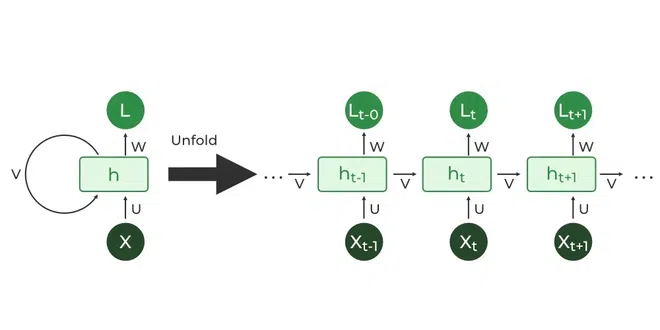
\includegraphics[width=0.55\textwidth]{rnn_image.png}
    \caption{Illustration du fonctionnement des Réseaux de Neurones Récurrents (RNN). Source : \url{https://miro.medium.com/v2/resize:fit:660/1*uLTBA8Myf6_IwtpfLr4Xpg.png}}
    \label{fig:rnn_architecture}
\end{figure}

\subsection{Long Short-Term Memory (LSTM)}

Les réseaux Long Short-Term Memory (\gls{lstm}) représentent une extension sophistiquée des réseaux de neurones récurrents (\gls{rnn}) traditionnels, conçue pour remédier à leurs limitations dans la capture des dépendances à long terme, notamment les problèmes de disparition ou d'explosion du gradient. Introduite par Hochreiter et Schmidhuber en 1997 \cite{hochreiter1997long}, l’architecture \gls{lstm} repose sur une cellule mémoire interne capable de conserver de l’information sur de longues séquences, contrôlée par un système de portes spécialisées.

À chaque instant temporel \( t \), les opérations fondamentales d'une cellule \gls{lstm} sont décrites par les équations suivantes :

\begin{align*}
f_t &= \sigma(W_f x_t + U_f h_{t-1} + b_f) \quad &\text{(Porte d'oubli)} \\
i_t &= \sigma(W_i x_t + U_i h_{t-1} + b_i) \quad &\text{(Porte d'entrée)} \\
\tilde{c}_t &= \tanh(W_c x_t + U_c h_{t-1} + b_c) \quad &\text{(État cellulaire candidat)} \\
c_t &= f_t \odot c_{t-1} + i_t \odot \tilde{c}_t \quad &\text{(Mise à jour de la cellule)} \\
o_t &= \sigma(W_o x_t + U_o h_{t-1} + b_o) \quad &\text{(Porte de sortie)} \\
h_t &= o_t \odot \tanh(c_t) \quad &\text{(État caché)}
\end{align*}

où :
\begin{itemize}
    \item \( x_t \) représente l’entrée à l’instant \( t \) ;
    \item \( h_{t-1} \) est l’état caché précédent ;
    \item \( f_t \), \( i_t \), \( o_t \) sont respectivement les vecteurs de la porte d’oubli, d’entrée et de sortie ;
    \item \( c_t \) désigne l’état de la cellule mémoire à l’instant \( t \) ;
    \item \( \tilde{c}_t \) est l’état cellulaire candidat proposé ;
    \item \( \sigma \) est la fonction sigmoïde, \( \tanh \) la tangente hyperbolique, et \( \odot \) désigne le produit élément par élément.
\end{itemize}

Cette structure permet aux \gls{lstm} de décider dynamiquement quelles informations conserver, mettre à jour ou émettre, offrant ainsi une capacité de mémorisation sélective très utile pour le traitement de séquences complexes. Grâce à cette flexibilité, les \gls{lstm} se sont imposés comme une référence dans de nombreuses tâches telles que la modélisation du langage, la traduction automatique, ou encore l’analyse de séries temporelles.

\begin{figure}[H]
    \centering
    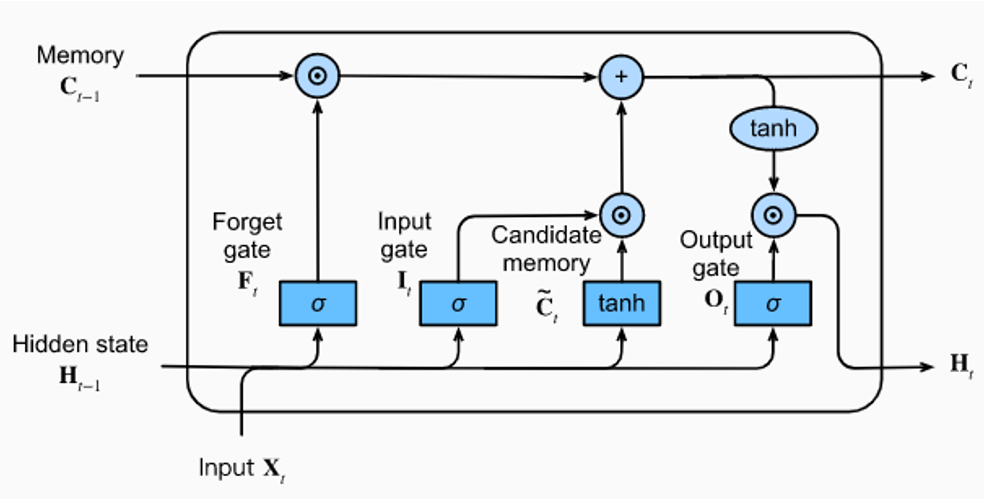
\includegraphics[width=0.55\textwidth]{lstm_image.png}
    \caption{Logique de l'architecture LSTM. Source : \url{https://sl.bing.net/bWWTQ1HkC7M}}
    \label{fig:lstm_architecture}
\end{figure}

\bigskip

\noindent Bien que puissants, les \gls{lstm} présentent une certaine complexité computationnelle en raison du nombre élevé de paramètres associés à leurs multiples portes. Pour proposer une alternative plus légère mais néanmoins efficace, la communauté a introduit une architecture simplifiée : le Gated Recurrent Unit (\gls{gru}).

\subsection{Gated Recurrent Unit (GRU)}

Le Gated Recurrent Unit (\gls{gru}) est une variante des \gls{rnn} introduite par Cho et al. en 2014 \cite{cho2014learning}, visant à réduire la complexité du modèle tout en maintenant des performances comparables à celles des \gls{lstm}. Contrairement aux \gls{lstm}, les \gls{gru} fusionnent les fonctions des portes d’oubli et d’entrée en une seule "porte de mise à jour", et n’utilisent pas d’état cellulaire distinct du vecteur caché. Cette simplification permet une convergence plus rapide et une efficacité accrue dans certaines tâches.

Les équations gouvernant une cellule \gls{gru} sont les suivantes :

\begin{align*}
z_t &= \sigma(W_z x_t + U_z h_{t-1} + b_z) \quad &\text{(Porte de mise à jour)} \\
r_t &= \sigma(W_r x_t + U_r h_{t-1} + b_r) \quad &\text{(Porte de réinitialisation)} \\
\tilde{h}_t &= \tanh(W_h x_t + U_h (r_t \odot h_{t-1}) + b_h) \quad &\text{(État candidat)} \\
h_t &= (1 - z_t) \odot h_{t-1} + z_t \odot \tilde{h}_t \quad &\text{(État caché)}
\end{align*}

où :
\begin{itemize}
    \item \( z_t \) est la porte de mise à jour ;
    \item \( r_t \) est la porte de réinitialisation ;
    \item \( \tilde{h}_t \) est l’état caché candidat ;
    \item \( h_t \) est l’état caché final de la cellule \gls{gru} à l’instant \( t \).
\end{itemize}

Cette architecture compacte permet aux \gls{gru} de s’adapter efficacement aux dépendances temporelles tout en limitant la charge computationnelle.

\begin{figure}[H]
    \centering
    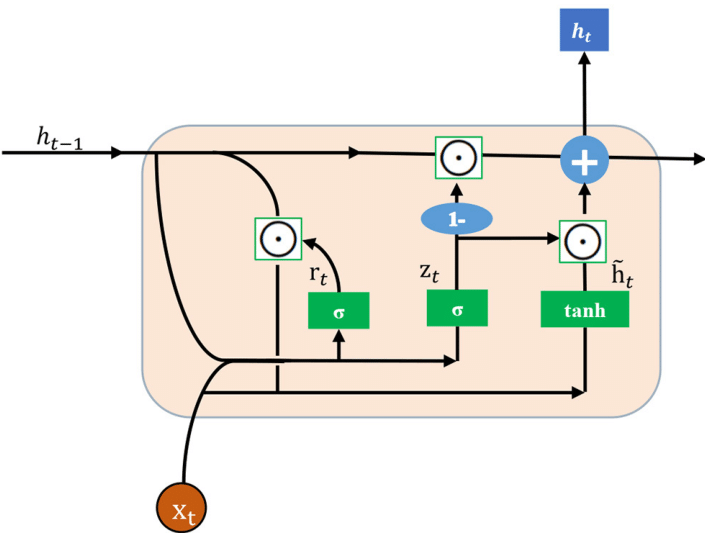
\includegraphics[width=0.45\textwidth]{gru_image.png}
    \caption{Illustration de l'unité récurrente à portes (GRU). Source : \url{https://sl.bing.net/bWWTQ1HkC7M}}
    \label{fig:gru_architecture}
\end{figure}

Cette architecture compacte permet aux \gls{gru} de s’adapter efficacement aux dépendances temporelles tout en limitant la charge computationnelle.

\vspace{0.5cm}

Cependant, malgré leur capacité à capturer des relations à long terme, les architectures séquentielles comme les \gls{lstm} et les \gls{gru} traitent les séquences de manière uniforme, sans accorder plus d’importance à certaines parties du texte qu’à d’autres. Pour pallier cette limitation, des mécanismes d’attention ont été introduits afin de permettre au modèle de se concentrer dynamiquement sur les éléments les plus pertinents de la séquence.

Parmi ces approches, le mécanisme d’attention proposé par Bahdanau et al. \cite{bahdanau2015neural} s’est imposé comme une extension efficace, initialement conçue pour la traduction automatique. Dans le cadre de ce mémoire, une adaptation simplifiée de cette attention est utilisée pour pondérer les sorties d’un \gls{gru} bidirectionnel dans une tâche de classification. La section suivante détaille ce mécanisme.

\section{Réseaux de Neurones Convolutionnels (CNN)}

Les réseaux de neurones convolutionnels (\gls{cnn}) sont des architectures largement utilisées en vision par ordinateur, mais leur application au traitement automatique du langage naturel (\gls{tln}) s’est révélée tout aussi prometteuse, notamment dans des tâches de classification de textes \cite{kim2014convolutional}. Leur principe repose sur l’extraction hiérarchique de caractéristiques à l’aide de filtres convolutifs glissants appliqués à une matrice représentant une séquence textuelle. 

Mathématiquement, l’opération de convolution discrète appliquée à une matrice d’entrée \( I \) et un noyau \( K \) est définie comme suit :

\begin{equation}
S(i, j) = (I * K)(i, j) = \sum_m \sum_n I(i + m, j + n) \cdot K(m, n)
\end{equation}

où \( S(i,j) \) désigne la sortie convoluée à la position \( (i,j) \), et les indices \( m,n \) parcourent les dimensions du filtre. Cette opération permet de détecter localement des motifs pertinents dans la structure du texte représenté sous forme matricielle.

Dans le cas d’un document textuel, chaque mot est d’abord représenté par un vecteur dense — soit appris durant l’entraînement, soit préentraîné (par exemple via \gls{glove} ou \gls{fasttext}). Ces vecteurs sont empilés pour former une matrice d’entrée de taille $L \times d$, où $L$ est la longueur du texte (ou le nombre de mots), et $d$ la dimension de l’embedding. Cette matrice est ensuite soumise à une \textit{couche de convolution}: des filtres (ou noyaux) glissent sur les lignes de la matrice, capturant des motifs locaux (comme des n-grammes) d’une taille fixée — par exemple, des fenêtres de 2, 3 ou 4 mots. Chaque filtre apprend à détecter une structure particulière (co-occurrence de termes, expressions spécifiques, tournures syntaxiques, etc.).

À la suite de cette convolution, une \textit{fonction d’activation} non linéaire, telle que la fonction ReLU (\textit{Rectified Linear Unit}), est généralement appliquée. Elle permet d’introduire de la non-linéarité dans le modèle et favorise la détection de motifs complexes.

Vient ensuite une \textit{opération de pooling}, souvent un max-pooling, qui réduit la dimension des représentations tout en conservant les informations les plus saillantes. Cette opération permet de rendre le modèle invariant aux petites variations dans la position des motifs détectés. Dans le cadre du \gls{tln}, cela revient à identifier les motifs les plus informatifs, quelle que soit leur position dans le texte.

Les représentations extraites par les filtres sont ensuite concaténées puis transmises à une ou plusieurs couches entièrement connectées (\textit{fully connected layers}), menant à une couche de sortie, généralement une \textit{softmax} (dans le cas de classification multiclasse) ou une \textit{sigmoid} (dans le cas binaire).

\begin{align}
\textit{sigmoid :} \quad \sigma(x) &= \frac{1}{1 + e^{-x}} \\[1em]
\textit{softmax :} \quad \text{softmax}(z_i) &= \frac{e^{z_i}}{\sum_{j=1}^{K} e^{z_j}} \quad \text{pour } i = 1, \dots, K
\end{align}

L’un des avantages majeurs des \gls{cnn} dans le traitement du texte est leur capacité à extraire des représentations discriminantes sans dépendre d’une modélisation explicite de l’ordre global de la séquence, tout en étant plus rapides à entraîner que les réseaux récurrents. En revanche, ils peinent parfois à capturer des dépendances à longue portée, raison pour laquelle ils sont souvent combinés à des architectures comme les \gls{gru} ou \gls{lstm}, comme c’est le cas dans ce mémoire avec les modèles hybrides \gls{cnn}-\gls{gru} et \gls{cnn}-\gls{lstm} \cite{zhou2015clstm}.

Ces architectures combinées bénéficient à la fois de la capacité des \gls{cnn} à extraire rapidement des motifs locaux, et de la capacité des réseaux récurrents à modéliser la dynamique temporelle et contextuelle des séquences. Cela en fait des candidats particulièrement pertinents pour la classification de textes biomédicaux, où les documents sont courts, denses en information, et s’appuient sur des structures linguistiques spécialisées.

\subsection{Mécanisme d’attention de Bahdanau}

Le mécanisme d'attention de Bahdanau, introduit dans le contexte de la traduction automatique neuronale \cite{bahdanau2015neural}, vise à surmonter les limitations des modèles séquentiels classiques qui compressent toute l’information d’une séquence dans un vecteur fixe. Cette compression peut être sous-optimale, notamment lorsque les séquences sont longues ou contiennent des informations dispersées.

L’attention permet au modèle de pondérer dynamiquement les éléments de la séquence en fonction de leur pertinence pour la tâche à accomplir. Autrement dit, au lieu de traiter toutes les parties d’un texte de manière égale, le modèle apprend à se concentrer davantage sur certaines parties pertinentes pour la prédiction.

Dans ce mémoire, une version simplifiée du mécanisme de Bahdanau est appliquée sur les sorties d’un \gls{gru} bidirectionnel. Concrètement, chaque sortie temporelle du \gls{gru} est transformée via un réseau feedforward afin de produire une importance (ou score d’attention). Ces scores sont ensuite normalisés via une fonction softmax pour obtenir des poids d’attention. Le vecteur de contexte est alors calculé comme une moyenne pondérée des états cachés de la séquence, où les poids reflètent la pertinence de chaque mot.

Le vecteur caché à un instant \( t \) dans un \gls{gru} bidirectionnel est défini comme la concaténation des vecteurs issus de la direction avant et arrière de la séquence :

\[
h_t = [\overrightarrow{h_t}; \overleftarrow{h_t}]
\]

où \( \overrightarrow{h_t} \) et \( \overleftarrow{h_t} \) sont respectivement les états cachés générés par les passes avant et arrière du \gls{gru}.

Le score d'attention pour chaque état caché à l'instant \( t \) est calculé comme suit :

\[
\text{score}_t = \mathbf{v}^\top \tanh(\mathbf{W} [\overrightarrow{h_t}; \overleftarrow{h_t}])
\]

L'importance relative de chaque élément de la séquence est ensuite calculée par une fonction softmax :

\[
\alpha_t = \frac{\exp(\text{score}_t)}{\sum_{t'} \exp(\text{score}_{t'})}
\]

Enfin, le vecteur de contexte, qui résume l'information pertinente des états cachés de la séquence, est obtenu par une somme pondérée des états cachés :

\[
\text{context} = \sum_t \alpha_t [\overrightarrow{h_t}; \overleftarrow{h_t}]
\]

Dans ces équations :

\begin{itemize}
    \item \( h_t \) est le vecteur caché à l’instant \( t \), qui est la concaténation des états cachés des directions avant et arrière;
    \item \( \alpha_t \) est le poids d’attention associé à l’état caché \( h_t \);
    \item \( \text{context} \) est le vecteur résultant, qui résume la séquence en mettant l’accent sur les éléments les plus pertinents.
\end{itemize}

Ce mécanisme permet au modèle d'exploiter à la fois les informations contextuelles antérieures et postérieures dans une séquence, ce qui est particulièrement utile pour des tâches comme la classification de textes biomédicaux, où un terme peut avoir un sens différent selon le contexte avant ou après son apparition.
\newline

Après avoir exploré le mécanisme d'attention de Bahdanau et son application dans des modèles séquentiels comme le \gls{gru} bidirectionnel, il est important de se pencher sur une autre composante essentielle dans les architectures de traitement du langage naturel : la représentation des mots et des phrases sous forme vectorielle. Ces représentations jouent un rôle fondamental dans la capture des relations sémantiques et contextuelles entre les termes.

Dans cette optique, plusieurs techniques de représentation vectorielle ont émergé pour mieux comprendre et modéliser le langage. Parmi les plus populaires, on trouve \gls{glove}, \gls{fasttext}, ainsi que des modèles de plus grande envergure spécifiquement conçus pour les domaines biomédicaux, tels que \gls{pubmedbert} et \gls{biobert}. Ces approches ont permis de dépasser les limites des représentations classiques, en intégrant à la fois des informations globales (comme les cooccurrences de mots) et des informations contextuelles plus fines.

La section suivante présente ces différentes techniques de représentation vectorielle, en mettant particulièrement l'accent sur leur application dans le domaine biomédical, où les termes sont souvent hautement spécialisés et contextuellement dépendants.

\vspace{0.5cm}
\section{Représentations de Vecteurs }

Les performances des modèles de traitement du langage naturel dépendent en grande partie de la manière dont les mots sont représentés numériquement. En effet, avant même l'application de modèles séquentiels ou de mécanismes d’attention, les textes doivent être transformés en vecteurs exploitables par les algorithmes d'apprentissage automatique.

Deux grandes familles de représentations vectorielles se distinguent : les \textit{word embeddings} statiques, qui attribuent un vecteur fixe à chaque mot indépendamment de son contexte, et les \textit{contextual embeddings}, qui ajustent dynamiquement les représentations en fonction du contexte d’apparition du mot dans la phrase.

Dans cette section, nous explorons tout d’abord les approches classiques basées sur les \textit{word embeddings}, notamment \gls{glove} et \gls{fasttext}, qui ont marqué une avancée significative dans la capture des relations sémantiques entre les mots. Ensuite, nous présentons des méthodes plus récentes et plus puissantes reposant sur des modèles de type Transformer, comme \gls{biobert} et \gls{pubmedbert}, qui produisent des représentations contextuelles particulièrement adaptées aux textes biomédicaux.

\subsection{Word Embeddings: GloVe and FastText}

Les \textit{word embeddings} statiques permettent de représenter chaque mot par un vecteur dense dans un espace continu de dimension réduite. Ces représentations sont apprises à partir de grands corpus de textes en exploitant les cooccurrences entre les mots. Deux des approches les plus influentes dans ce domaine sont \gls{glove} et \gls{fasttext}.

\begin{figure}[H]
    \centering
    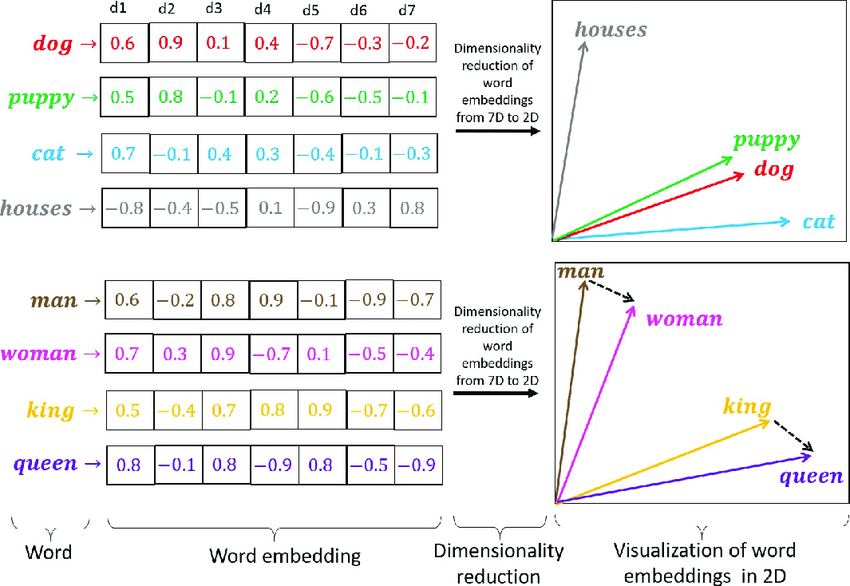
\includegraphics[width=0.65\textwidth]{we.png}
    \caption{Illustration du principe des \textit{word embeddings} : les mots similaires sont projetés dans des régions proches de l’espace vectoriel. Source : \url{https://sl.bing.net/jumSq5RbE1Q}}
    \label{fig:word_embeddings}
\end{figure}

\subsubsection{FastText}

\gls{fasttext} \cite{bojanowski2017enriching}, développé par Facebook \gls{ia} Research, est une extension de \gls{w2v}, une méthode d’apprentissage de représentations vectorielles des mots développée par Mikolov et al. Contrairement à \gls{glove} ou \gls{w2v}, qui considèrent chaque mot comme une unité atomique, \gls{fasttext}  représente un mot comme la somme des vecteurs de ses sous-unités, appelées \textit{n-grammes} de caractères. Formellement, si un mot \( w \) est composé de n-grammes \( g_1, g_2, \dots, g_K \), alors sa représentation vectorielle \( \mathbf{v}_w \) est définie comme :

\[
\mathbf{v}_w = \sum_{k=1}^{K} \mathbf{z}_{g_k}
\]

où \( \mathbf{z}_{g_k} \) est le vecteur associé au n-gramme \( g_k \).

Par exemple, le mot `chat'' avec des trigrammes (n=3), serait représenté par les n-grammes suivants : \_ch'', cha'', hat'', at\_''. \gls{fasttext} ajoute également des délimiteurs de mot (\_'' au début et à la fin) pour distinguer les positions dans le mot.

Cette représentation permet au modèle de partager l'information entre les mots ayant des morphologies similaires, ce qui le rend robuste aux mots rares ou inconnus (\textit{out-of-vocabulary}). De plus, FastText est capable de produire des vecteurs pour des mots absents du vocabulaire d’entraînement, tant que leurs sous-unités ont été observées.

En conservant les propriétés sémantiques de \gls{w2v} tout en capturant des régularités morphologiques (préfixes, suffixes, racines), FastText est particulièrement adapté à des domaines spécialisés comme le biomédical, où les termes sont souvent longs, composés et rares.

\subsubsection{GloVe}

\gls{glove} \cite{pennington2014glove} est une méthode d'apprentissage non supervisée qui combine les avantages des approches basées sur les fenêtres locales (comme \gls{w2v}) et des méthodes statistiques globales. Elle repose sur la construction d'une matrice de cooccurrence entre les mots dans un corpus, où chaque entrée \( X_{ij} \) correspond au nombre de fois que le mot \( j \) apparaît dans le contexte du mot \( i \).

L’objectif du modèle est d’apprendre des vecteurs \( w_i \) et \( \tilde{w}_j \) pour chaque mot \( i \) et contexte \( j \) de sorte que leur produit scalaire approche le logarithme de \( X_{ij} \) :

\[
w_i^\top \tilde{w}_j + b_i + \tilde{b}_j \approx \log(X_{ij})
\]

où \( b_i \) et \( \tilde{b}_j \) sont des biais appris. En optimisant cette relation sur toutes les paires de mots fréquents, \gls{glove} produit des embeddings qui capturent efficacement les relations sémantiques et analogiques, comme illustré par :

\[
\vec{\text{roi}} - \vec{\text{homme}} + \vec{\text{femme}} \approx \vec{\text{reine}}
\]

Ces deux méthodes fournissent une base solide pour représenter les mots avant l'application de modèles de traitement plus complexes. Toutefois, leurs limites résident dans leur incapacité à désambiguïser les mots selon le contexte, ce qui a motivé l’émergence des représentations contextuelles abordées dans la section suivante.

\begin{figure}[H]
    \centering
    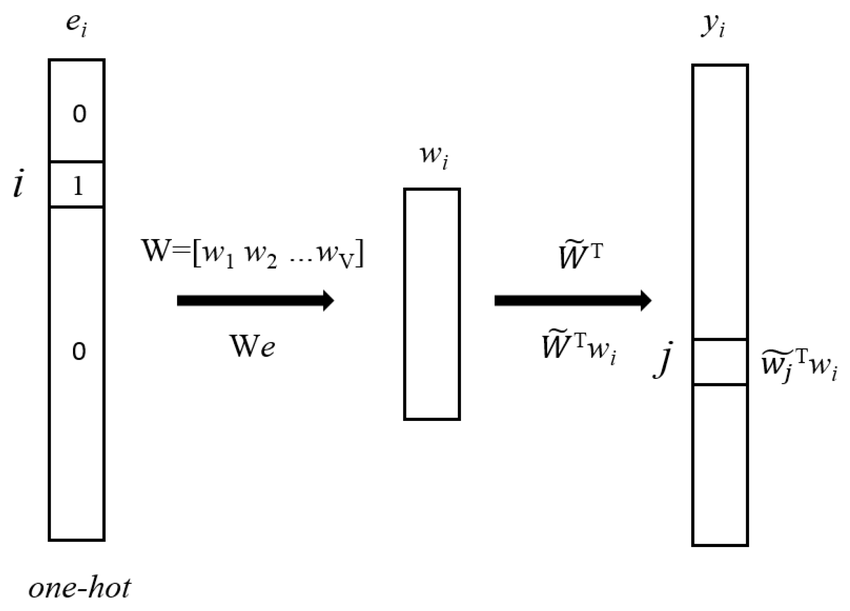
\includegraphics[width=0.35\textwidth]{glove.png}
    \caption{Architecture du modèle GloVe, illustrant la construction des vecteurs à partir des cooccurrences. L'entrée est une représentation \textit{one-hot} d’un mot à un instant donné. Les matrices d'intégration des mots sont utilisées comme matrices de poids, et la sortie du modèle est un vecteur obtenu par produit scalaire entre les vecteurs de mots. Source : \url{https://www.researchgate.net/figure/The-model-architecture-of-GloVe-The-input-is-a-one-hot-representation-of-a-word-The_fig1_337461648}}
    \label{fig:glove_architecture}
\end{figure}

% Ici, développe BioBERT et PubMedBERT
\subsection{Contextual Embeddings: BioBERT and PubMedBERT}

Bien que les \textit{word embeddings} statiques comme \gls{glove} et \gls{fasttext} aient significativement amélioré la qualité des représentations lexicales, ils présentent une limitation majeure : chaque mot y est associé à un vecteur unique, quelle que soit sa signification dans le contexte. Cela pose problème pour les mots polysémiques ou ambigus, fréquents dans le langage naturel et particulièrement critiques en biomédecine.

Pour pallier cette limite, les modèles récents s'appuient sur des architectures de type Transformer, capables de produire des représentations contextuelles dynamiques. Dans ces modèles, un même mot peut être représenté par des vecteurs différents selon le contexte dans lequel il apparaît.

Dans cette section, nous explorons deux représentations contextuelles spécialement entraînées sur des corpus biomédicaux : \gls{biobert} et \gls{pubmedbert}. Ces modèles, basés sur l’architecture de \gls{bert}, capturent des nuances sémantiques essentielles pour des tâches complexes telles que l’extraction d’informations biomédicales, la classification de documents scientifiques, ou encore la normalisation de concepts médicaux.

\subsection{BioBERT comme vecteur de plongement contextuel}

\gls{biobert} est une variante du modèle \gls{bert} spécialement préentraînée sur des corpus biomédicaux, tels que PubMed Abstracts et PMC Full-text articles \cite{lee2020biobert}. À l’instar de BERT, il génère des \textit{plongements de mots contextuels} (\textit{contextual embeddings}) : chaque mot est représenté par un vecteur dense qui dépend non seulement du mot lui-même, mais aussi de son contexte environnant.

Contrairement aux méthodes de plongement statique comme \gls{glove} ou \gls{w2v}, qui assignent un seul vecteur à chaque mot indépendamment du contexte, \gls{biobert} est capable de moduler dynamiquement les représentations en fonction des autres tokens présents dans la même phrase. Cela est rendu possible grâce à son architecture fondée sur des couches de type Transformer exploitant le mécanisme d’auto-attention (\textit{self-attention}).

Le mécanisme de self-attention calcule les dépendances entre tous les tokens d’une séquence, permettant à chaque mot de se représenter en fonction des autres :

\begin{equation}
\textit{Attention}(Q, K, V) = \text{softmax} \left( \frac{QK^{T}}{\sqrt{d_k}} \right) V
\end{equation}

où $Q$, $K$ et $V$ sont respectivement les matrices de requêtes, de clés et de valeurs dérivées des représentations d’entrée, et $d_k$ est la dimension des vecteurs clés. Cette opération permet au modèle de pondérer les interactions entre chaque paire de mots, capturant ainsi efficacement les relations sémantiques et syntaxiques, même à longue distance.

Le processus débute par une tokenisation via WordPiece (figure.~\ref{fig:wordpiece}), qui découpe les mots en sous-unités, puis par un encodage positionnel et segmentaire. Les tokens sont ensuite traités par plusieurs couches de Transformer, où le mécanisme d’auto-attention calcule, pour chaque token, une représentation vectorielle tenant compte de tous les autres tokens de la séquence. La sortie de ces couches est une série de vecteurs contextuels riches, adaptés à des tâches spécifiques comme la classification, la reconnaissance d’entités biomédicales ou l’extraction de relations.

\begin{figure}[H]
    \centering
    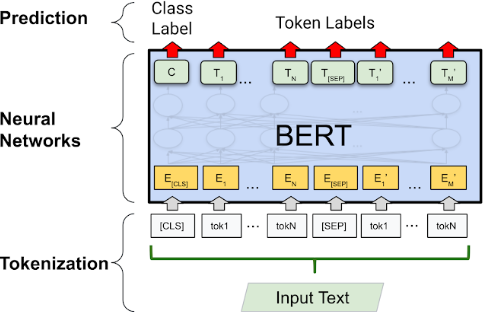
\includegraphics[width=0.7\textwidth]{tokenization_bert.png}
    \caption{Illustration du processus de tokenisation WordPiece suivi par l'encodage et les couches Transformer. Source : \url{https://research.googleblog.com/2021/12/a-fast-wordpiece-tokenization-system.html}}
    \label{fig:wordpiece}
\end{figure}

\gls{biobert} conserve l’architecture bidirectionnelle de \gls{bert} — chaque couche reçoit à la fois le contexte gauche et droit de chaque mot — mais il est initialisé avec les poids de \gls{bert} de base et affiné (\textit{fine-tuned}) sur de grands corpus biomédicaux. Cette spécialisation rend \gls{biobert} particulièrement performant dans les tâches du domaine de la santé : classification de textes biomédicaux, reconnaissance d'entités nommées, question-réponse clinique, etc.

\subsection{PubMedBERT comme vecteur de plongement contextuel}

\gls{pubmedbert} est une variante du modèle \gls{bert} qui a été préentraînée spécifiquement sur des textes biomédicaux extraits de la base de données PubMed, un des plus grands corpus de la littérature scientifique dans le domaine médical. PubMedBERT se distingue par le fait qu'il a été conçu pour mieux capturer les spécificités lexicales et les relations complexes qui existent dans les textes médicaux et biologiques, en particulier dans les domaines de la recherche biomédicale et des publications cliniques \cite{gu2020domain}. 

À l’instar de \gls{biobert}, \gls{pubmedbert} génère des \textit{plongements de mots contextuels} (\textit{contextual embeddings}) qui varient selon le contexte dans lequel les mots apparaissent. Cependant, \gls{pubmedbert} se distingue par son préentraînement exclusif sur les articles de PubMed, ce qui lui permet de mieux comprendre la terminologie et la sémantique propres à la biomédecine. En effet, \gls{pubmedbert} est capable de générer des vecteurs denses qui intègrent des informations spécifiques à la terminologie médicale, permettant ainsi des performances accrues dans des tâches comme l’extraction d’entités biomédicales, la classification de publications scientifiques ou encore l’analyse de relations entre concepts médicaux.

Le modèle s'appuie sur l’architecture Transformer et le mécanisme d’auto-attention pour produire des représentations vectorielles dépendant du contexte des mots, tout comme \gls{biobert}. La tokenisation initiale est réalisée à l’aide de WordPiece, un processus de découpage de mots en sous-unités qui permet une meilleure gestion des mots rares ou composés. Cela permet au modèle de traiter efficacement la grande variété de termes techniques rencontrés dans la littérature biomédicale.

Le processus de traitement des tokens dans \gls{pubmedbert} suit une approche similaire à celle de \gls{biobert} : une tokenisation via WordPiece (cf. Fig.~\ref{fig:wordpiece}) permet de découper les termes médicaux complexes en sous-unités, suivie par l'application d'un encodage positionnel et segmentaire. Les tokens sont ensuite passés par plusieurs couches de Transformer où chaque token est représenté par un vecteur contextuel calculé grâce au mécanisme d’auto-attention, prenant en compte l'ensemble des tokens de la séquence. La sortie de ces couches est une série de vecteurs contextuels qui sont utilisés pour des tâches spécifiques, telles que la classification de textes biomédicaux, l'extraction d'informations cliniques ou l'identification d'entités nommées dans des publications scientifiques.

Ainsi \gls{pubmedbert} est une solution puissante pour les applications biomédicales, où la compréhension fine de la terminologie médicale et scientifique est essentielle. Son préentraînement sur PubMed, combiné à l’architecture Transformer, lui permet d’obtenir de solides résultats dans des tâches complexes telles que la reconnaissance d'entités biomédicales, la classification de documents scientifiques et l’extraction d’informations cliniques, tout en prenant en compte les particularités linguistiques du domaine médical.

\section{Visualisation des représentations des données avec t-SNE}
\label{sec:tsne}

La visualisation des représentations vectorielles est une étape importante pour mieux comprendre comment un modèle de traitement du langage naturel apprend à distinguer les différentes classes à partir des données textuelles. Dans ce projet, nous utilisons l’algorithme \gls{tsne}~\cite{van2008visualizing} afin de projeter des vecteurs de haute dimension dans un espace bidimensionnel pour une visualisation intuitive.

\gls{tsne} (t-distributed Stochastic Neighbor Embedding) repose sur une modélisation probabiliste de la proximité entre points. Dans l’espace d’origine (de haute dimension), la similarité entre deux points $x_i$ et $x_j$ est définie comme une probabilité conditionnelle $p_{j|i}$, donnée par :

\begin{equation}
p_{j|i} = \frac{\exp(-\|x_i - x_j\|^2 / 2\sigma_i^2)}{\sum_{k \neq i} \exp(-\|x_i - x_k\|^2 / 2\sigma_i^2)}
\end{equation}

La probabilité symétrique conjointe est ensuite définie par :

\begin{equation}
p_{ij} = \frac{p_{j|i} + p_{i|j}}{2n}
\end{equation}

où $n$ est le nombre total de points. Dans l’espace projeté de faible dimension, une distribution $q_{ij}$ est définie sur les points projetés $y_i$ et $y_j$ en utilisant une distribution de Student à une seule liberté (plus lourde en queue que la Gaussienne) :

\begin{equation}
q_{ij} = \frac{(1 + \|y_i - y_j\|^2)^{-1}}{\sum_{k \neq l} (1 + \|y_k - y_l\|^2)^{-1}}
\end{equation}

L’objectif de \gls{tsne} est alors de minimiser la divergence de Kullback-Leibler (KL) entre ces deux distributions de similarité :

\begin{equation}
\mathcal{L} = KL(P \| Q) = \sum_{i \neq j} p_{ij} \log \left( \frac{p_{ij}}{q_{ij}} \right)
\end{equation}

Cette minimisation est effectuée par descente de gradient, et permet de préserver les structures locales des données — les paires de points proches en haute dimension restant proches dans l’espace 2D projeté.

Appliqué à différentes étapes du pipeline, \gls{tsne} permet d’obtenir une représentation visuelle des données telles qu’elles sont perçues par le modèle — que ce soit à l’entrée (par exemple, les embeddings de type \gls{glove} ou \gls{biobert}) ou à travers les activations intermédiaires après passage dans les couches du modèle (\gls{lstm}, attention, etc.).

L’interprétation des projections \gls{tsne} repose sur la conservation de la structure locale des données. En d’autres termes, si deux points sont proches dans l’espace projeté, ils étaient probablement aussi proches dans l’espace original à haute dimension. Ainsi, une bonne séparation visuelle entre groupes (ou classes) dans la carte \gls{tsne} peut indiquer que le modèle a appris des représentations discriminantes. À l’inverse, un chevauchement important peut signaler que les classes sont peu séparables dans l’espace appris, ce qui peut se traduire par des erreurs de classification.

Dans le cadre de ce travail, \gls{tsne} nous a permis de visualiser les regroupements de données issus de différentes classes, d'identifier des zones de confusion potentielle entre classes, et d'observer l'évolution des représentations apprises par le modèle au cours de l'entraînement.

Cette visualisation n’est pas simplement illustrative : elle offre une lecture qualitative du comportement du modèle et peut orienter des choix méthodologiques, par exemple en suggérant l’introduction de techniques de rééquilibrage ou l’ajustement de l’architecture si les classes restent difficilement séparables.

\section{L'apprentissage par petites touches dans le cadre du TALN : définitions, méthodes et défis}

L'apprentissage par petites touches \gls{fsl} représente une approche où les modèles doivent apprendre efficacement à partir de seulement quelques exemples par classe, un scénario couramment rencontré dans des contextes où il est difficile d'obtenir une quantité suffisante de données annotées. Cette approche est particulièrement utile en \gls{tln}, où les jeux de données peuvent être rares ou difficiles à annoter manuellement, comme dans les applications spécifiques à des domaines tels que la biomédecine ou le droit.

\subsection{Définitions et Concepts}

L'apprentissage par petites touches repose sur l'idée qu'un modèle peut apprendre des tâches complexes en utilisant très peu d'exemples. Cette capacité est essentielle pour surmonter les limitations des méthodes traditionnelles qui nécessitent de grandes quantités de données annotées pour obtenir de bonnes performances. Dans ce cadre, un k-shot se réfère au nombre d'exemples utilisés par classe pour entraîner un modèle. Par exemple, dans le cadre d'un problème de 5-shot learning, le modèle est entraîné avec cinq exemples par classe.

L'un des concepts clés du \gls{fsl} est la capacité des modèles à généraliser à partir de peu d'exemples. Cela nécessite de fortes capacités d'abstraction et de transfert de connaissances acquises lors de pré-entraînements sur des jeux de données plus larges, comme le montrent les travaux sur les architectures basées sur \gls{bert} et ses variantes \cite{devlin2019bert, lee2020biobert, lu2020pubmedbert}.

\subsection{Méthodes et Techniques}

Les méthodes de \gls{fsl} en \gls{tln} incluent des approches telles que le meta-learning (apprentissage de l'apprentissage), qui permet aux modèles de se former rapidement sur de nouvelles tâches avec peu d'exemples. Des techniques comme Matching Networks \cite{vinyals2016matching}, Prototypical Networks \cite{snell2017prototypical} et MAML (Model-Agnostic Meta-Learning) \cite{finn2017model} sont couramment utilisées. Ces méthodes se basent sur des mécanismes permettant au modèle d'apprendre à partir de peu d'exemples, en optimisant la capacité à adapter rapidement le modèle à de nouvelles tâches.

Les Transformers comme \gls{bert} \cite{devlin2019bert} et ses dérivés, tels que \gls{biobert} \cite{lee2020biobert} ou \gls{pubmedbert} \cite{lu2020pubmedbert}, ont été particulièrement efficaces dans les tâches de \gls{fsl} en TAL, car ils sont capables de capturer des représentations contextuelles riches et adaptatives. Ces modèles sont souvent pré-entraînés sur de vastes corpus et sont ensuite adaptés (fine-tunés) pour des tâches spécifiques avec peu d'exemples.

\subsection{Défis de l'Apprentissage par Petites Touches}

L'un des défis majeurs de l'apprentissage par petites touches est la généralisation. Le modèle doit être capable de faire des prédictions fiables malgré le nombre limité d'exemples d'entraînement. Cette difficulté est accentuée dans des domaines spécifiques comme la biomédecine, où la richesse sémantique et la polysémie des termes rendent le modèle susceptible de faire des erreurs si le contexte n'est pas bien compris \cite{jin2019recurrent, zhang2020biowordvec}. Les techniques telles que l'entraînement multitâche et le transfert d'apprentissage peuvent aider à surmonter ces obstacles en tirant parti de l'information présente dans des tâches ou des domaines similaires.

Le contraste entre les classes dans un jeu de données de Few-Shot peut également être un défi. Les modèles doivent être capables de distinguer des exemples très similaires tout en étant robustes aux variations dans les données d'entrée. Des approches comme l'augmentation de données et des techniques de régularisation peuvent être utiles pour améliorer la robustesse des modèles en \gls{fsl}. 

\section{Problèmes de déséquilibre des classes et techniques d’adaptation}
\label{sec:class-imbalance}

Le déséquilibre des classes est un problème fréquent dans la classification de textes biomédicaux, où certaines classes sont surreprésentées tandis que d’autres, souvent plus rares mais cliniquement importantes, sont sous-représentées. Cette disparité peut fortement biaiser l’apprentissage du modèle, qui tend alors à privilégier la classe majoritaire au détriment de la précision sur les classes minoritaires. Pour y remédier, plusieurs techniques d’adaptation ont été développées, parmi lesquelles des méthodes de rééchantillonnage et des stratégies de pondération des classes dans la fonction de perte. Ces techniques sont particulièrement pertinentes dans des contextes à faible volume de données ou à fort déséquilibre, comme en biomédecine.

\subsection{Méthodes de rééchantillonnage}

Les méthodes de rééchantillonnage visent à modifier la distribution des données afin de compenser le déséquilibre entre les classes. On distingue principalement deux approches :
\begin{itemize}
    \item le \textbf{suréchantillonnage}, qui augmente artificiellement la proportion des exemples minoritaires ;
    \item le \textbf{sous-échantillonnage}, qui réduit la taille des classes majoritaires pour équilibrer la distribution.
\end{itemize}

Bien que les deux types de méthodes soient couramment utilisés dans la littérature, notre projet se concentre exclusivement sur les techniques de \textbf{suréchantillonnage}. Ce choix repose sur une revue d’articles spécialisés dans l’apprentissage sur données déséquilibrées, notamment dans le domaine biomédical, où la conservation des données majoritaires est souvent cruciale pour préserver la richesse des cas cliniques. Par ailleurs, les méthodes de suréchantillonnage permettent d’enrichir la classe minoritaire sans altérer la structure globale du jeu de données.

Parmi les approches de suréchantillonnage, nous avons retenu deux techniques largement reconnues : \gls{smote} (Synthetic Minority Over-sampling Technique)~\cite{chawla2002smote} et sa variante Borderline-\gls{smote}~\cite{han2005borderline}. Ces méthodes ont démontré leur efficacité dans plusieurs études pour améliorer la performance des modèles sur des jeux de données fortement déséquilibrés.
\subsubsection{\gls{smote} — \textbf{Synthetic Minority Over-sampling Technique}}

\gls{smote}~\cite{chawla2002smote} est une méthode de suréchantillonnage qui vise à résoudre les problèmes de déséquilibre de classes dans les jeux de données, en particulier ceux où les classes minoritaires sont sous-représentées. Contrairement à des approches plus simples, comme la duplication aléatoire d’exemples minoritaires, \gls{smote} génère de nouveaux exemples synthétiques par interpolation, ce qui introduit une plus grande diversité dans les données.

Le principe fondamental de \gls{smote} consiste à sélectionner aléatoirement un des $k$ plus proches voisins d’un échantillon minoritaire, puis à créer un nouvel exemple le long du segment qui relie ces deux points dans l’espace des caractéristiques. Formellement, si $x_i$ est un exemple minoritaire et $x_i^{(NN)}$ l’un de ses voisins proches, un nouvel exemple synthétique $x_{\text{new}}$ est généré selon la formule :

\begin{equation}
x_{\text{new}} = x_i + \delta \cdot (x_i^{(NN)} - x_i), \quad \text{où } \delta \sim \mathcal{U}(0,1)
\end{equation}

où $\delta$ est un facteur de pondération aléatoire, tiré d’une distribution uniforme. Cette interpolation linéaire produit des instances qui sont proches des données existantes, tout en enrichissant l’espace des caractéristiques de la classe minoritaire de manière plus fluide que des duplications exactes.

Cette technique présente plusieurs avantages : elle réduit le risque de surapprentissage, améliore la définition des frontières de décision, et permet aux classifieurs d'apprendre à mieux généraliser dans les zones de faible densité. Elle est particulièrement pertinente dans les contextes biomédicaux où certaines conditions rares ou maladies spécifiques sont peu représentées dans les données.

Cependant, \gls{smote} présente également des limites. Notamment, il peut créer des instances synthétiques non représentatives si les voisins utilisés se trouvent près des frontières entre classes, ce qui peut introduire du bruit. De plus, en étendant artificiellement la minorité, il peut exacerber le chevauchement entre classes si le problème initial n'est pas linéairement séparable. Des variantes comme Borderline-\gls{smote} ont été proposées pour pallier ces inconvénients en adaptant la génération d’exemples aux zones les plus ambiguës.

Le principe de \gls{smote} est illustré dans la Figure~\ref{fig:smote_algo}, qui présente l'algorithme sous forme de pseudocode. Celui-ci détaille les étapes de génération d'exemples synthétiques par interpolation aléatoire entre un échantillon minoritaire et ses voisins les plus proches. Cette méthode peut être combinée à d’autres techniques, comme le sous-échantillonnage de la classe majoritaire ou la pondération de la fonction de perte, afin d’optimiser les performances sur des jeux de données déséquilibrés.

\begin{figure}[H]
    \centering
    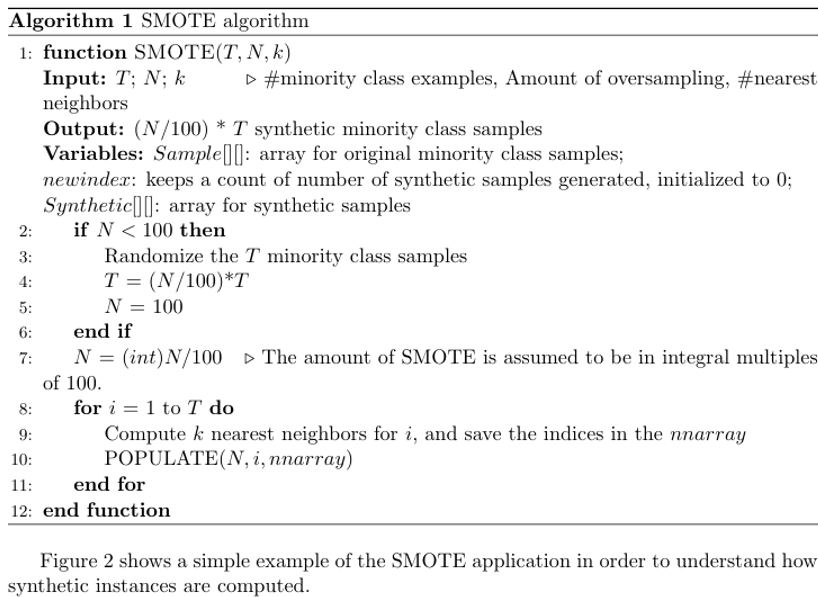
\includegraphics[width=0.8\textwidth]{smote.png}
    \caption{Algorithme \gls{smote} : génération d'exemples synthétiques à partir des voisins proches d'une instance minoritaire. Adapté de \cite{chawla2002smote}.}
    \label{fig:smote_algo}
\end{figure}

\subsubsection{Borderline-SMOTE}

Borderline-\gls{smote}~\cite{han2005borderline} est une variante de \gls{smote} qui cible spécifiquement les exemples situés à proximité des frontières de décision, c’est-à-dire les zones les plus susceptibles d’entraîner des erreurs de classification. Dans les applications sensibles comme le diagnostic médical, où les erreurs sur des cas ambigus peuvent être critiques, cette méthode renforce la capacité du modèle à discriminer correctement les classes dans les situations les plus complexes. Elle fonctionne en identifiant les échantillons minoritaires qui sont entourés de nombreux exemples de la classe majoritaire (situations "borderline") et en générant de nouveaux exemples à partir de ceux-là, afin de densifier ces zones critiques de l’espace de décision.

\section{Pondération des classes dans la fonction de perte}

La pondération des classes dans la fonction de perte est une méthode utilisée pour compenser le déséquilibre des classes en attribuant un poids plus élevé aux classes minoritaires. Cette approche permet de corriger le biais induit par un déséquilibre des classes sans altérer les données elles-mêmes. Elle est particulièrement utile dans les domaines où certaines classes sont cliniquement importantes mais sous-représentées, comme en biomédecine \cite{Chawla2002SMOTE} ou en science politique \cite{King2001Logit}.

Soit $y_i$ l'étiquette réelle de l'échantillon $i$, et $\hat{y}_i$ la prédiction du modèle pour cet échantillon. La fonction de perte classique pour une classification binaire (par exemple, l'entropie croisée) est donnée par :

$$
\mathcal{L}_\text{classique} = - \sum_{i=1}^{N} \left[ y_i \log(\hat{y}_i) + (1 - y_i) \log(1 - \hat{y}_i) \right]
$$

Cependant, dans le cas de classes déséquilibrées, cette fonction de perte peut entraîner un modèle qui favorise la classe majoritaire. Pour résoudre ce problème, on modifie cette fonction de perte en attribuant des poids $w_1$ et $w_0$ aux classes 1 et 0, respectivement. La fonction de perte pondérée devient alors :

$$
\mathcal{L}_\text{pondérée} = - \sum_{i=1}^{N} \left[ w_1 \cdot y_i \log(\hat{y}_i) + w_0 \cdot (1 - y_i) \log(1 - \hat{y}_i) \right]
$$

où $w_1$ et $w_0$ sont les poids associés respectivement aux classes 1 et 0. Ces poids peuvent être définis en fonction de la fréquence des classes dans le jeu de données. 


\vspace{1em}
Dans un problème multi-classe, chaque étiquette $y_i$ appartient à l'une des classes possibles, disons $C = \{1, 2, \dots, K\}$, où $K$ est le nombre total de classes. Le modèle prédit une probabilité $\hat{y}_i$ pour chaque classe $k$, c'est-à-dire $\hat{y}_i = P(\hat{y} = k | x_i)$ \cite{Han2005Borderline}.

La fonction de perte classique pour la classification multi-classe, telle que l'entropie croisée, est donnée par :

$$
\mathcal{L}_\text{classique} = - \sum_{i=1}^{N} \sum_{k=1}^{K} y_{ik} \log(\hat{y}_{ik})
$$

où $y_{ik}$ est l'étiquette binaire pour l'échantillon $i$ et la classe $k$ (soit 1 si $x_i$ appartient à la classe $k$, sinon 0), et $\hat{y}_{ik}$ est la probabilité prédite pour cette classe.

Pour adapter la fonction de perte au déséquilibre des classes dans un cadre multi-classe, on attribue un poids $w_k$ à chaque classe $k$. La fonction de perte pondérée devient alors :

$$
\mathcal{L}_\text{pondérée} = - \sum_{i=1}^{N} \sum_{k=1}^{K} w_k \cdot y_{ik} \log(\hat{y}_{ik})
$$

où $w_k$ est le poids associé à la classe $k$.

Comme pour le cas binaire, ces poids peuvent être définis de manière inversement proportionnelle à la fréquence des classes dans le jeu de données. Les poids peuvent être calculés de différentes manières, en fonction du déséquilibre des classes. 

La perte focale, proposée par Lin et al. \cite{Lin2017Focal}, cette méthode introduit un facteur de modulation pour focaliser l'apprentissage sur les exemples difficiles à classer, tout en conservant une pondération selon la classe (où $\gamma$ est un paramètre de focalisation) :
$$
\mathcal{L}_\text{local} = - \sum_{i=1}^{N} \sum_{k=1}^{K} w_k \cdot (1 - \hat{y}_{ik})^\gamma \cdot y_{ik} \log(\hat{y}_{ik})
$$.

\chapter{État de l’art}

\section{Panorama des méthodes de classification des textes biomédicaux}

La classification automatique de textes biomédicaux constitue un domaine central du traitement automatique du langage naturel (\gls{tln}), particulièrement essentiel pour des applications comme l'analyse des publications scientifiques, l'extraction d'informations cliniques ou encore les systèmes de soutien au diagnostic. Ce domaine a évolué parallèlement aux progrès réalisés en apprentissage automatique, et en particulier en apprentissage profond. L'objectif de cette section est de présenter l'évolution des approches de classification des textes biomédicaux, en se concentrant sur les travaux majeurs qui ont influencé ce domaine, tout en soulignant les motivations qui ont conduit à la réalisation de ce travail de thèse.

Dans les premières années de développement de la classification automatique des textes, les modèles étaient principalement basés sur des représentations simples comme le \textit{bag-of-words}. Ces approches traditionnelles incluaient également des méthodes comme les machines à vecteurs de support (SVM) ou encore les classifieurs Naïve Bayes. Ces techniques, bien que solides, peinaient à capturer les relations contextuelles complexes entre les termes, essentielles dans le domaine biomédical. Les corpus biomédicaux, souvent caractérisés par une forte spécialisation du vocabulaire et une grande ambiguïté sémantique, nécessitaient une approche plus sophistiquée, capable de comprendre ces relations subtiles.

L’évolution vers des modèles séquentiels a commencé dans les années 2010 avec l'émergence des réseaux neuronaux récurrents (\gls{rnn}), et plus particulièrement les variantes \gls{lstm} et \gls{gru}. Ces modèles ont permis de mieux modéliser les dépendances temporelles et contextuelles des mots dans une séquence de texte. En effet, dans des domaines comme la biologie ou la médecine, les relations entre les mots ne sont pas indépendantes, mais dépendent du contexte dans lequel ils apparaissent. Les \gls{rnn}, introduits par Elman (1990)~\cite{elman1990finding}, ont été les premiers modèles capables de traiter des séquences de données en capturant ces dépendances, mais ils souffraient d'un problème majeur : le phénomène du \textit{vanishing gradient} qui rendait difficile l'apprentissage sur de longues séquences. C’est dans ce contexte que les \gls{lstm}, proposés par Hochreiter et Schmidhuber (1997)~\cite{hochreiter1997long}, ont vu le jour, en introduisant des mécanismes de mémoire qui ont grandement amélioré la gestion de ces longues dépendances dans les données.

Les \gls{gru}, introduits plus récemment par Cho et al. (2014)~\cite{cho2014learning}, ont simplifié l'architecture des \gls{lstm}, tout en conservant des performances similaires, avec l'avantage de nécessiter moins de paramètres. Ces avancées ont permis une meilleure gestion des dépendances contextuelles, et ont donc trouvé une application naturelle dans le domaine biomédical, où il est crucial de capturer les relations entre les différentes entités médicales présentes dans un texte.

Parallèlement, les représentations de mots statiques comme \gls{w2v} et \gls{glove}, ainsi que des embeddings spécifiques au domaine comme BioWordVec~\cite{zhang2020biowordvec}, ont permis d’améliorer la représentation sémantique des termes. Ces modèles ont aidé à surmonter la limitation des représentations basées uniquement sur le comptage de mots, en fournissant des vecteurs denses qui capturent les relations sémantiques entre les mots.

Cependant, c'est avec l'essor des modèles basés sur les Transformers que la classification des textes biomédicaux a connu un véritable tournant. Les modèles tels que \gls{biobert}~\cite{lee2020biobert} et \gls{pubmedbert}~\cite{gupta2021pubmedbert}, préentraînés sur des corpus biomédicaux spécifiques, ont permis de capturer des relations contextuelles beaucoup plus fines, en prenant en compte l’ensemble du contexte autour d’un terme. Ces modèles ont permis de réaliser des avancées significatives dans la classification des textes médicaux, en particulier dans des tâches complexes comme l'extraction d'entités médicales et la reconnaissance de relations entre différentes entités.

À partir de 2018, la recherche s’est également orientée vers des scénarios plus complexes comme l’apprentissage par faible supervision (\gls{fsl}), où les modèles sont capables de s'adapter à des ensembles de données peu annotées ou déséquilibrées. Des techniques d'adaptation de domaine et de méta-apprentissage ont également été explorées pour permettre une meilleure généralisation et une plus grande robustesse des modèles face à des variations de langage ou des domaines spécifiques.

En nous appuyant sur ces différentes avancées, notre travail s'inscrit dans cette continuité de la recherche. Nous proposons de combiner ces techniques de manière innovante pour surmonter les défis spécifiques de la classification des textes biomédicaux, notamment la gestion du vocabulaire spécialisé, l'ambiguïté des termes et le déséquilibre des classes dans les corpus. Ce travail s’inspire largement des modèles séquentiels, en particulier des \gls{lstm}, \gls{gru} et des architectures récentes comme \gls{biobert}, pour aborder la classification dans ce domaine avec des solutions adaptées et performantes.

\subsection{Approches classiques}

Avant l’émergence des réseaux neuronaux profonds, la classification de textes biomédicaux reposait principalement sur des méthodes d’apprentissage automatique traditionnelles. Ces dernières s’appuyaient sur des représentations vectorielles creuses (\textit{sparse}), telles que le modèle \textit{Bag-of-Words} ou la pondération TF-IDF (\textit{Term Frequency–Inverse Document Frequency}), qui ignorent totalement l’ordre des mots ainsi que leur structure syntaxique ou sémantique. Les modèles classiques comme le classifieur Naïve Bayes, les machines à vecteurs de support (SVM) ou encore les arbres de décision étaient fréquemment utilisés, recevant en entrée ces vecteurs issus de représentations lexicales simples.

Par exemple, Japkowicz et Stephen (2002) \cite{japkowicz2002class} ont mis en évidence les limites de ces approches dans les contextes de déséquilibre des classes, phénomène courant dans les données biomédicales. De même, King et Zeng (2001) \cite{King2001Logit} ont étudié les performances dégradées des modèles de régression logistique face aux événements rares, ce qui pose un défi dans la classification de documents médicaux peu représentés. Si ces méthodes présentent l’avantage d’être interprétables et rapides à entraîner, elles ne permettent pas de capturer les relations sémantiques entre mots ni leur contexte d’apparition dans la phrase.

Ainsi, les modèles de classification de textes biomédicaux ont considérablement évolué avec les progrès du traitement du langage naturel et de l'apprentissage profond. Nous allons dans la suite nous concentrer sur les travaux spécifiques qui ont influencé la manière dont les modèles actuels sont utilisés dans le domaine biomédical. Dans les sections suivantes, nous explorerons des études précises, notamment celles portant sur l’application des \gls{lstm}, \gls{rnn} et des architectures plus complexes, pour mieux comprendre leurs contributions à la classification des textes dans le contexte biomédical. Ces travaux, tirés de la littérature, serviront de base à la conception et à l'implémentation de la méthode proposée dans ce travail de thèse.

Nous commencerons par examiner en détail les recherches ayant intégré des architectures récurrentes pour traiter des données biomédicales spécifiques, avant de nous intéresser aux récentes approches hybrides qui combinent plusieurs types de réseaux pour maximiser les performances de classification. Ces perspectives ouvriront la voie à la présentation de la méthodologie spécifique développée dans ce travail.

\subsection{Finding Structure in Time}

L’article fondateur de Jeffrey L. Elman intitulé \textit{Finding Structure in Time}~\cite{elman1990finding} marque une étape décisive dans l’évolution des modèles séquentiels pour le traitement du langage naturel. Dans ce travail, Elman introduit une architecture de réseau neuronal récurrent simple (SRN, \textit{Simple Recurrent Network}) destinée à apprendre des régularités temporelles dans des séquences linguistiques. Il ne s’agit pas simplement d’un développement technique, mais d’une démonstration empirique que des structures grammaticales et lexicales implicites peuvent émerger de l’exposition à des données séquentielles non annotées.

Le SRN fonctionne selon un principe fondamental : à chaque pas de temps $t$, l’entrée $x_t$ est combinée à un état de contexte $h_{t-1}$ (provenant de la couche cachée à l’instant précédent) pour produire un nouvel état caché $h_t$. Formellement, cela peut être représenté par :

\begin{equation}
h_t = \sigma(W_{xh} x_t + W_{hh} h_{t-1} + b_h), \quad y_t = \text{softmax}(W_{hy} h_t + b_y)
\end{equation}

où $\sigma$ est une fonction d’activation non linéaire (comme $\tanh$), $W_{xh}$, $W_{hh}$, et $W_{hy}$ sont des matrices de poids, et $y_t$ est la prédiction effectuée à l’instant $t$. La capacité du réseau à conserver l’information temporelle repose uniquement sur le passage récurrent de l’état caché, ce qui introduit une forme de mémoire.

Elman teste son modèle sur des tâches croissantes de complexité, démontrant que même un réseau récurrent simple peut développer des représentations internes qui capturent des structures linguistiques profondes :

\paragraph{Structure dans les séquences de lettres.} Le SRN est d’abord entraîné sur des séquences de lettres générées selon des règles probabilistes simples. Rapidement, le réseau parvient à prédire les lettres suivantes avec une précision significative, montrant qu’il a appris des régularités orthographiques implicites. Ce résultat suggère que l’apprentissage prédictif peut conduire à l’émergence de motifs structurés dans des flux continus de symboles.

\paragraph{Découverte implicite de la notion de mot.} Une expérience emblématique de l’article consiste à soumettre le SRN à un flux continu de caractères sans séparation explicite entre les mots. De façon remarquable, le réseau identifie implicitement les frontières lexicales, en capturant des statistiques de transition entre les lettres. Cette capacité d’induction structurelle sans supervision préfigure les modèles modernes d’apprentissage non supervisé.

\paragraph{Identification de classes lexicales à partir de l’ordre des mots.} Dans une tâche plus complexe, Elman expose le réseau à des séquences de mots respectant une grammaire artificielle. Le SRN apprend non seulement à prédire les éléments suivants mais organise les représentations internes de manière à regrouper les mots selon leur rôle grammatical (noms, verbes, déterminants, etc.). Ainsi, les représentations latentes révèlent l’acquisition spontanée de catégories syntaxiques.

Ce travail met en lumière plusieurs concepts clés : l’apprentissage distribué de représentations, l’importance de la mémoire dans le traitement séquentiel, et la capacité des réseaux à découvrir des structures hiérarchiques implicites. Il propose également des perspectives développementales : Elman postule que les contraintes temporelles et la capacité limitée de mémoire jouent un rôle dans la structuration progressive du langage chez l’enfant. Cette hypothèse a donné lieu à des travaux en psycholinguistique computationnelle, suggérant une convergence entre les processus d’apprentissage machine et cognitifs.

Cependant, le SRN souffre de limitations importantes, notamment le problème du gradient qui disparaît lors de la rétropropagation à travers le temps (\textit{vanishing gradient problem}), ce qui nuit à l’apprentissage de dépendances à long terme. Ces limites ont motivé l’émergence d’architectures plus robustes comme les réseaux LSTM~\cite{hochreiter1997long}, conçus spécifiquement pour surmonter ces difficultés.

En définitive, l’article de Elman constitue une pierre angulaire du développement des réseaux neuronaux pour le traitement du langage naturel, en montrant qu’un apprentissage prédictif simple peut induire une compréhension structurelle du langage. Ce paradigme reste central dans les architectures contemporaines, qu’il s’agisse des modèles récurrents, convolutionnels ou transformeurs.

\begin{figure}[H]
\centering
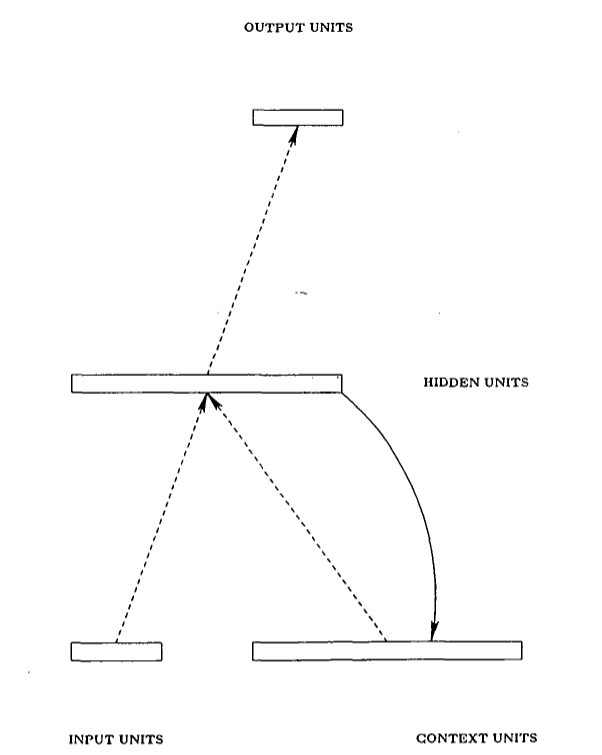
\includegraphics[width=0.4\linewidth]{rnn_elman.png}
\caption{Réseau récurrent simple selon Elman~\cite{elman1990finding}. Les activations de la couche cachée sont transférées à la couche de contexte avec un poids fixe de 1. Les connexions en pointillés sont les poids entraînables du réseau.}
\label{fig:elman_rnn}
\end{figure}

Enfin, l’article souligne que l’apprentissage efficace de structures hiérarchiques impose une contrainte sur la mémoire à court terme du réseau. Elman propose même une solution inspirée du développement humain : commencer l’apprentissage avec des séquences simples et augmenter progressivement leur complexité, une idée connue aujourd’hui sous le nom de \textit{curriculum learning}.

\subsection{Text Classification Improved by Integrating Bidirectional LSTM with Two-dimensional Max Pooling}

L’article de Zhou et al.~\cite{zhou2015text} propose une architecture innovante combinant un réseau bidirectionnel \gls{lstm} (BiLSTM) avec une opération de max pooling bidimensionnelle, dans le but explicite d'améliorer la classification des textes.

Le modèle repose d'abord sur un encodage bidirectionnel via un BiLSTM, qui permet de capturer simultanément les dépendances passées et futures dans une séquence. Contrairement aux \gls{rnn} classiques, le BiLSTM conserve des informations contextuelles des deux directions, ce qui est particulièrement utile dans le traitement des textes où les relations sémantiques peuvent dépendre de mots situés avant et après un terme cible.

Les auteurs utilisent des vecteurs de mots préentraînés \gls{glove}, construits à partir de 6 milliards de tokens issus de Wikipedia 2014 et du corpus Gigaword 5. Les mots absents de ce vocabulaire sont initialisés aléatoirement à l’aide d’une distribution uniforme dans l’intervalle $[-0{,}25, 0{,}25]$. Ces embeddings sont ensuite affinés pendant l’entraînement du modèle afin d’adapter les représentations lexicales à la tâche de classification.

L’innovation majeure introduite par les auteurs réside dans l’utilisation du \textit{2D max pooling} appliqué à la sortie du BiLSTM. Cette technique, inspirée des réseaux convolutionnels, permet d’extraire les caractéristiques les plus saillantes sur l’ensemble de la séquence encodée, réduisant ainsi le bruit et augmentant la robustesse du classifieur final. Grâce à cette combinaison, le modèle est capable de capturer non seulement des dépendances temporelles mais aussi des interactions locales plus fines entre les représentations cachées générées par le BiLSTM.

\begin{figure}[H]
    \centering
    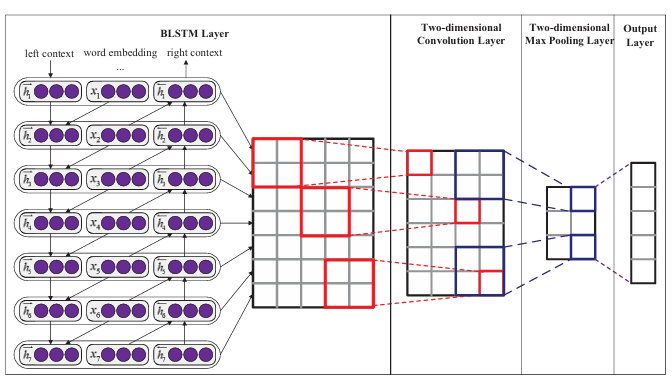
\includegraphics[width=0.7\textwidth]{bilstm.png}
    \caption{Architecture du modèle BLSTM-2DCNN pour une séquence de sept mots. Les vecteurs de mots ont une dimension de 3, et le BiLSTM comporte 5 unités cachées. La hauteur et la largeur des filtres convolutifs et des opérations de max pooling sont fixées à 2~\cite{zhou2015text}.}
    \label{fig:bilstm-arch}
\end{figure}

Les expérimentations, menées sur six jeux de données de classification textuelle (dont SST-1, SST-2, TREC, etc.), montrent que le modèle BLSTM-2DCNN surpasse non seulement les modèles \gls{rnn}, \gls{cnn} classiques, et les RecNN (Recursive Neural Networks), mais aussi les variantes proches comme le BLSTM-2DPooling ou le DSCNN (Deep Structured Convolutional Neural Network) proposé par Zhang et al.~(2016). Notamment, il atteint la meilleure précision sur les ensembles de données SST-1 et SST-2, souvent utilisés comme références dans les tâches de classification fine de sentiments.

Une analyse de sensibilité conduite sur SST-1 démontre également que l’utilisation de filtres convolutifs de grande taille permet de capturer davantage de motifs sémantiques complexes, ce qui peut améliorer significativement les performances. Ces résultats soulignent l’efficacité de la combinaison du BiLSTM avec des stratégies de réduction dimensionnelle en 2D, qui permettent de conserver à la fois les informations temporelles et les dimensions vectorielles issues des représentations de mots.

Ainsi, l’approche BLSTM-2DCNN représente une avancée notable dans la classification des textes, en offrant un compromis efficace entre richesse de représentation et simplicité de l’architecture, ce qui la rend particulièrement prometteuse pour des domaines complexes comme la biomédecine ou le juridique.

\subsection{BioBERT : Un modèle de langage préentraîné pour le domaine biomédical}

L’émergence des modèles de langage préentraînés comme \gls{bert} a révolutionné le traitement automatique du langage naturel (\gls{tln}), notamment en réduisant le besoin d’architectures spécifiques à chaque tâche grâce à un mécanisme d'attention bidirectionnelle. Cependant, malgré ses performances générales, \gls{bert} montre des limites dans les domaines spécialisés comme le biomédical, où le vocabulaire, la terminologie et les structures syntaxiques diffèrent notablement du langage général.

Pour répondre à cette problématique, Lee et al. (2020) ont introduit \gls{biobert}, une variante de \gls{bert} spécifiquement préentraînée sur de larges corpus biomédicaux, notamment les abstracts de PubMed (4,5 milliards de mots) et les articles en texte intégral de PMC (13,5 milliards de mots). L’objectif était d’adapter les représentations sémantiques de \gls{bert} au domaine biomédical, afin d'améliorer ses performances sur les tâches telles que la reconnaissance d’entités nommées (NER), l’extraction de relations (RE), et le question answering (QA).

\paragraph{Architecture de BioBERT.} \gls{biobert} reprend intégralement l'architecture de BERT\textsubscript{BASE}, composée de \textit{12 couches de transformeurs}, \textit{768 dimensions pour les représentations cachées}, \textit{12 têtes d’attention}, et environ \textit{110 millions de paramètres}. Il n’y a donc aucune modification structurelle par rapport à \gls{bert} ; l'amélioration provient uniquement du corpus de pré-entraînement et du vocabulaire spécialisé. \gls{biobert} est initialisé avec les poids de BERT\textsubscript{BASE} et continue le pré-entraînement avec un objectif de modélisation de langue masquée (MLM) sur les textes biomédicaux.

\begin{figure}[H]
    \centering
    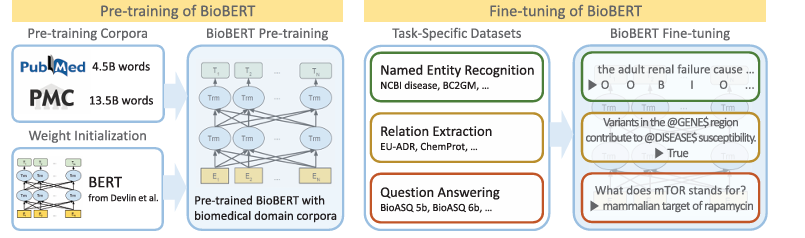
\includegraphics[width=0.75\textwidth]{biobert.png}
    \caption{Vue d'ensemble de la phase de pré-entraînement et de fine-tuning de BioBERT~\cite{lee2020biobert}.}
    \label{fig:biobert_architecture}
\end{figure}

Cette figure~\ref{fig:biobert_architecture} illustre le processus global de construction de \gls{biobert}, structuré en deux phases principales : le pré-entraînement et le fine-tuning. La première phase consiste à continuer l’entraînement du modèle BERT\textsubscript{BASE} sur de larges corpus spécialisés tels que PubMed et PMC, à l’aide de la tâche de modélisation de langage masqué (Masked Language Modeling). Cette étape vise à adapter les représentations linguistiques du modèle aux spécificités du domaine biomédical, sans modifier l’architecture initiale de \gls{bert}. La seconde phase, le fine-tuning, correspond à l’adaptation du modèle à des tâches précises du \gls{tln} biomédical telles que la reconnaissance d’entités nommées (NER), l’extraction de relations (RE) et le question answering (QA). Cette visualisation met en évidence que les gains de performance de \gls{biobert} ne proviennent pas d’un changement architectural, mais exclusivement du type et de la qualité du corpus utilisé lors de l’entraînement, soulignant ainsi l’importance des données spécialisées dans le succès de l’adaptation des modèles de langage préentraînés.

L'étude de Lee et al. a comparé différentes combinaisons de corpus pour le pré-entraînement, démontrant que plus le corpus est biomédical, meilleures sont les performances du modèle :

\begin{table}[H]
\centering
\caption{Pré-entraînement de BioBERT selon les corpus textuels utilisés~\cite{lee2020biobert}}
\scriptsize
\resizebox{0.6\textwidth}{!}{%
\begin{tabular}{|l|l|}
\hline
\textbf{Modèle} & \textbf{Corpus utilisé} \\
\hline
BERT (baseline) & Wiki + Books \\
BioBERT (+PubMed) & Wiki + Books + PubMed \\
BioBERT (+PMC) & Wiki + Books + PMC \\
BioBERT (+PubMed + PMC) & Wiki + Books + PubMed + PMC \\
\hline
\end{tabular}%
}
\end{table}

L’évaluation a été menée sur plusieurs benchmarks de référence en \gls{tln}biomédical. Parmi ceux-ci :
\begin{itemize}
    \item \textit{NER (Named Entity Recognition)} : sur des jeux de données comme NCBI Disease, BC5CDR, JNLPBA, BioNLP13CG.
    \item \textit{RE (Relation Extraction)} : sur ChemProt et GAD.
    \item \textit{QA (Question Answering)} : sur BioASQ, une compétition d'extraction de réponses médicales à partir de PubMed.
\end{itemize}

\begin{figure}[H]
    \centering
    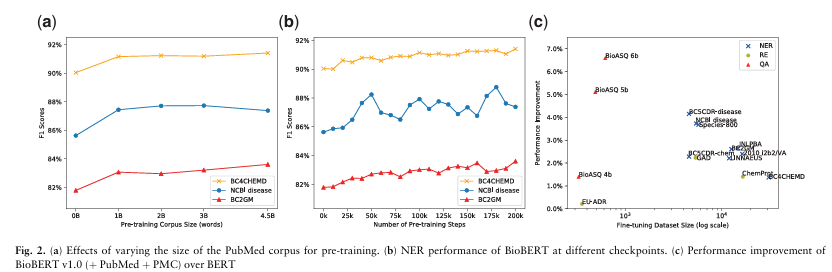
\includegraphics[width=0.8\textwidth]{result_biobert.png}
    \caption{(a) Effet de la taille du corpus PubMed sur le pré-entraînement. (b) Performances NER de BioBERT à différents checkpoints. (c) Amélioration obtenue par BioBERT v1.0 (PubMed + PMC) par rapport à BERT~\cite{lee2020biobert}.}
    \label{fig:biobert_results}
\end{figure}

Les auteurs de \gls{biobert} ont conduit une série d'expérimentations pour évaluer l'impact du volume de données biomédicales utilisées lors du pré-entraînement. Les résultats, illustrés dans la figure~\ref{fig:biobert_results}(a), montrent que l’augmentation progressive de la taille du corpus PubMed entraîne une amélioration significative des performances du modèle sur plusieurs tâches de reconnaissance d’entités nommées (NER). Plus précisément, les scores F1 augmentent de manière notable pour les jeux de données NCBI Disease, BC4CHEMD et BC5CDR. Toutefois, au-delà d’un certain seuil — environ 4,5 milliards de mots — les performances tendent à se stabiliser, indiquant que le modèle atteint une saturation en termes de bénéfices apportés par des données supplémentaires. Cela souligne qu’un pré-entraînement sur un large corpus biomédical est bénéfique, bien que l’effet marginal décroisse à mesure que le corpus s’élargit.

La figure~\ref{fig:biobert_results}(b) met en évidence l’évolution des performances de \gls{biobert} au cours du pré-entraînement, en fonction du nombre de pas d’apprentissage. On observe que les résultats s’améliorent globalement avec l’augmentation du nombre de pas, ce qui démontre la capacité du modèle à continuer à apprendre des représentations linguistiques pertinentes sur le long terme. Cette progression est particulièrement marquée pour certaines tâches comme celle du NCBI Disease, pour laquelle les fluctuations sont plus visibles mais tendent vers une convergence performante. Cette observation corrobore l'idée que le pré-entraînement prolongé, lorsqu’il est effectué sur un corpus spécialisé, permet une spécialisation fine du modèle aux subtilités du langage biomédical.

Enfin, la figure~\ref{fig:biobert_results}(c) compare directement les performances de \gls{biobert} par rapport au modèle \gls{bert} généraliste. L’amélioration est mesurée en fonction de la taille du jeu de données utilisé pour le fine-tuning, ce dernier étant représenté en échelle logarithmique. Il ressort de cette analyse que les gains les plus significatifs sont obtenus sur les tâches de question answering (QA), notamment sur les différentes versions de BioASQ, où l'amélioration dépasse les 6~\%. Les tâches de NER bénéficient également d’un gain notable, généralement compris entre 2~\% et 4~\%. En revanche, les tâches d’extraction de relations (RE) affichent des gains plus modestes, bien qu’ils restent constants. Un aspect particulièrement intéressant est que les plus fortes améliorations sont observées sur les jeux de données de petite taille, ce qui souligne l’intérêt de \gls{biobert} dans des contextes où les ressources annotées sont limitées. Ainsi, ces résultats confirment la pertinence du pré-entraînement sur des données spécialisées, et démontrent que la qualité du corpus joue un rôle central dans l’adaptation efficace des modèles de langage aux domaines spécifiques.


\newpage

\chapter{Architectures et expériences}

\chapter{Architectures et expériences}

\section{Sources et structuration des données}

Les données utilisées dans cette étude proviennent de \textbf{PubMed}, une base de données biomédicale de référence regroupant des millions d’articles scientifiques publiés entre \textbf{1950 et 2024}. Les textes exploités correspondent aux résumés (\textit{abstracts}) d’articles académiques, incluant des publications de recherche, des essais cliniques et des études épidémiologiques. Tous les documents sont publics, dé-identifiés, et ne contiennent aucune donnée personnelle ou confidentielle.

Afin d’évaluer la robustesse et la généralisabilité des modèles de classification de texte, deux tâches distinctes ont été définies : une tâche \textbf{de classification binaire} et une tâche \textbf{de classification multiclasses}. Ces deux configurations expérimentales permettent de tester le comportement des modèles dans des contextes de complexité croissante, allant d’une discrimination simple entre deux catégories à une classification fine entre plusieurs pathologies.

La première tâche est une classification binaire visant à distinguer les articles liés au \textit{paludisme} (malaria) de ceux traitant d'autres maladies, en l’occurrence la \textit{maladie d’Alzheimer} et la \textit{dengue}. Le jeu de données associé contient environ \textit{30\,000 résumés}, avec une répartition fortement déséquilibrée en faveur de la classe « malaria ». Cette configuration simule un cas courant en santé publique, où certaines maladies bénéficient d’une attention disproportionnée dans la littérature scientifique.

La seconde tâche, plus complexe, consiste en une classification multiclasses dans laquelle chaque résumé est associé à l’une des \textit{neuf classes pathologiques} sélectionnées. Celles-ci incluent à la fois des maladies infectieuses (comme la tuberculose, le choléra ou Ebola) et non infectieuses (comme la leucémie, l’asthme, ou la mucoviscidose). Le corpus totalise environ \textit{43\,000 résumés}, là encore avec un fort déséquilibre inter-classes, certaines maladies étant bien plus représentées que d'autres dans la base de données.

Le choix de ces deux tâches repose sur la volonté de capturer à la fois des dynamiques simples et complexes de classification. La tâche binaire permet d’analyser le comportement des modèles dans un contexte épuré mais déséquilibré, tandis que la tâche multiclasses met à l’épreuve leur capacité à discriminer finement entre plusieurs entités sémantiquement proches ou très diverses. Ce double cadre expérimental est ainsi particulièrement pertinent pour modéliser les défis réels rencontrés dans la classification automatique de documents biomédicaux.

\section{Analyse exploratoire des données}

Avant de procéder au prétraitement des données, il est essentiel de comprendre leur structure, leur distribution et les éventuelles anomalies qui pourraient influencer la performance des modèles. L'analyse exploratoire des données (EDA) consiste à examiner les caractéristiques des résumés biomédicaux présents dans le corpus, notamment la répartition des classes, la longueur des résumés, et la fréquence des termes spécifiques.

Les étapes suivantes illustrent les résultats de l'EDA réalisés sur notre jeu de données.

\subsection{Répartition des classes}
La distribution des classes est fortement déséquilibrée, avec une surreprésentation de la classe \textit{malaria} dans la tâche binaire. De même, certaines pathologies comme la tuberculose et le choléra dominent dans la tâche multiclasses.

\subsection{Analyse de la longueur des résumés}
La longueur des résumés varie considérablement, certains étant relativement courts (moins de 100 mots), tandis que d'autres peuvent dépasser les 500 mots. Cette variation pourrait affecter l'efficacité des modèles de classification et nécessite une approche particulière pour le prétraitement.

\subsection{Identification des termes fréquents}
L'examen des termes les plus fréquents dans les résumés permet d'identifier des mots-clés spécifiques à chaque pathologie, ainsi que des termes communs dans la littérature biomédicale. Ces informations sont cruciales pour comprendre les patterns du texte et orienter les stratégies de prétraitement.




































\section{Métriques d’évaluation pour la classification de textes biomédicaux}

Dans le cadre de la classification de textes, en particulier dans des domaines spécialisés comme la biomédecine, le choix des métriques d’évaluation est crucial pour mesurer de manière fiable les performances des modèles. Comme l’ont souligné Saito et al.~\cite{saito2015precision}, les métriques traditionnelles comme l’\textbf{accuracy} peuvent être trompeuses dans des contextes de déséquilibre de classes, ce qui est fréquent en biomédecine ou en apprentissage avec peu d’exemples.

L’\textbf{accuracy}, définie comme le rapport entre les prédictions correctes et le nombre total de prédictions, reste la métrique la plus utilisée. Toutefois, son efficacité diminue fortement en cas de classes déséquilibrées. Comme l’ont noté Japkowicz et Stephen~\cite{japkowicz2002class}, un modèle peut obtenir une accuracy élevée simplement en prédisant la classe majoritaire, sans réellement apprendre à discriminer les classes minoritaires.

Pour remédier à ces limites, la \textbf{balanced accuracy} a été introduite comme alternative plus équitable. Elle est définie comme la moyenne des rappels (\textit{recall}) pour chaque classe, permettant ainsi une évaluation robuste, même lorsque certaines classes sont fortement sous-représentées~\cite{brodersen2010balanced}.

La \textbf{precision} et le \textbf{recall} sont deux métriques complémentaires : la première mesure la proportion de vrais positifs parmi les prédictions positives, tandis que la seconde mesure la proportion de vrais positifs correctement identifiés parmi tous les éléments réellement positifs. Le \textbf{F1-score}, leur moyenne harmonique, est recommandé dans les travaux récents sur la classification de textes en contexte médical, notamment par Jin et al.~\cite{jin2019recurrent}, car il pénalise les déséquilibres entre précision et rappel. 

Enfin l'\gls{auc} (Area Under the Curve), et plus précisément l’AUC-ROC (Receiver Operating Characteristic), est une métrique utilisée pour évaluer la capacité d’un modèle à distinguer entre les classes positives et négatives. Elle mesure l’aire sous la courbe ROC, qui trace le taux de vrais positifs en fonction du taux de faux positifs. Une AUC proche de 1 indique un excellent pouvoir discriminant, tandis qu’une AUC de 0{,}5 correspond à une performance aléatoire. Comme l’ont montré Saito et Rehmsmeier~\cite{saito2015precision}, dans les contextes de fort déséquilibre de classes – comme en biomédecine –, l’AUC-PR (Precision-Recall) est souvent plus informative que l’AUC-ROC, car elle se concentre davantage sur les performances en ce qui concerne la classe positive rare.



































































































\newpage
\begin{thebibliography}{99}

\bibitem{bahdanau2015neural}
D. Bahdanau, K. Cho, and Y. Bengio, 
\textit{Neural Machine Translation by Jointly Learning to Align and Translate}, 
International Conference on Learning Representations (ICLR), 2015. 
\url{https://arxiv.org/abs/1409.0473}

\bibitem{bengio1994learning}
Y. Bengio, et al., 
\textit{Learning long-term dependencies with gradient descent is difficult}, 
IEEE Transactions on Neural Networks, vol. 5, no. 2, pp. 157–166, 1994.

\bibitem{bojanowski2017enriching}
P. Bojanowski, E. Grave, A. Joulin, and T. Mikolov, 
\textit{Enriching word vectors with subword information}, 
Transactions of the Association for Computational Linguistics, vol. 5, pp. 135–146, 2017. 
\url{https://aclanthology.org/Q17-1010/}

\bibitem{brodersen2010balanced}
K. H. Brodersen, C. S. Ong, K. E. Stephan, and J. M. Buhmann, 
\textit{The balanced accuracy and its posterior distribution}, 
20th International Conference on Pattern Recognition, 2010.

\bibitem{cho2014learning}
K. Cho, B. van Merriënboer, D. Bahdanau, and Y. Bengio, 
\textit{Learning phrase representations using RNN encoder-decoder for statistical machine translation}, 
arXiv preprint arXiv:1406.1078, 2014. 
\url{https://arxiv.org/abs/1406.1078}

\bibitem{devlin2019bert}
J. Devlin, M. W. Chang, K. Lee, and K. Toutanova, 
\textit{BERT: Pre-training of deep bidirectional transformers for language understanding}, 
NAACL-HLT 2019, pp. 4171–4186, 2019. 
\url{https://arxiv.org/abs/1810.04805}

\bibitem{elman1990finding}
J. L. Elman, 
\textit{Finding structure in time}, 
Cognitive Science, vol. 14, no. 2, pp. 179–211, 1990.

\bibitem{finn2017model}
C. Finn, P. Abbeel, and S. Levine, 
\textit{Model-Agnostic Meta-Learning for Fast Adaptation of Deep Networks}, 
ICML 2017, pp. 1126–1135, 2017. 
\url{https://arxiv.org/abs/1703.03400}

\bibitem{gupta2021pubmedbert}
A. Gupta and A. Agarwal, 
\textit{PubMedBERT: A pre-trained biomedical language representation model for PubMed abstracts}, 
arXiv preprint arXiv:2102.09714, 2021. 
\url{https://arxiv.org/abs/2102.09714}

\bibitem{he2009learning}
H. He, X. L. Chen, and D. W. Song, 
\textit{Learning from imbalanced data}, 
Proceedings of the IEEE International Conference on Data Mining, 2009.

\bibitem{hochreiter1997long}
S. Hochreiter and J. Schmidhuber, 
\textit{Long short-term memory}, 
Neural Computation, vol. 9, no. 8, pp. 1735–1780, 1997.

\bibitem{lu2020pubmedbert}
Z. Lu et al., 
\textit{PubMedBERT: Pre-trained language model for biomedical text mining}, 
[Journal/Conference], 2020. 
\url{https://arxiv.org/abs/2007.XXX}

\bibitem{jia2019deep}
L. Jia, et al., 
\textit{Deep learning for medical text mining: A survey}, 
Journal of Biomedical Informatics, vol. 96, pp. 103–118, 2019.

\bibitem{jin2019recurrent}
Q. Jin, B. Dhingra, X. Liu, W. Cohen, and E. Hovy, 
\textit{Recurrent neural network models for disease name recognition using domain-invariant features}, 
In Proceedings of the BioNLP 2019 Workshop, pp. 1–10, 2019.

\bibitem{lee2020biobert}
J. Lee, W. Yoon, S. Kim, D. Kim, and C. H. So, 
\textit{BioBERT: A pre-trained biomedical language representation model for biomedical text mining}, 
Bioinformatics, vol. 36, no. 4, pp. 1234–1240, 2020. 
\url{https://doi.org/10.1093/bioinformatics/btz682}

\bibitem{mikolov2010recurrent}
T. Mikolov, M. Karafiát, L. Burget, J. Černocký, and S. Khudanpur, 
\textit{Recurrent neural network based language model}, 
In Interspeech, vol. 2, pp. 1045–1048, 2010.

\bibitem{mikolov2018advances}
T. Mikolov and others, 
\textit{Advances in pretraining models}, 
Journal of Machine Learning, vol. 10, pp. 1–10, 2018.

\bibitem{pennington2014glove}
J. Pennington, R. Socher, and C. D. Manning, 
\textit{GloVe: Global Vectors for Word Representation}, 
In Proceedings of the 2014 Conference on Empirical Methods in Natural Language Processing (EMNLP), pp. 1532–1543, 2014. 
\url{https://aclanthology.org/D14-1162/}

\bibitem{snell2017prototypical}
J. Snell, K. Swersky, and R. Zemel, 
\textit{Prototypical Networks for Few-shot Learning}, 
NeurIPS 2017, pp. 4077–4087, 2017. 
\url{https://arxiv.org/abs/1703.05175}

\bibitem{vinyals2016matching}
O. Vinyals, C. Blundell, T. Lillicrap, D. Wierstra, and D. Silver, 
\textit{Matching Networks for One-Shot Learning}, 
NeurIPS 2016, pp. 3630–3638, 2016. 
\url{https://arxiv.org/abs/1606.04080}

\bibitem{yin2017comparative}
W. Yin, K. Kann, M. Yu, and H. Schütze, 
\textit{Comparative study of CNN and RNN for natural language processing}, 
arXiv preprint arXiv:1702.01923, 2017. 
\url{https://arxiv.org/abs/1702.01923}

\bibitem{zhang2020biowordvec}
Y. Zhang, Q. Chen, Z. Yang, H. Lin, and Z. Lu, 
\textit{BioWordVec, improving biomedical word embeddings with subword information and MeSH}, 
Scientific Data, vol. 6, no. 52, 2020. 
\url{https://doi.org/10.1038/s41597-019-0055-0}

\bibitem{saito2015precision}
T. Saito and M. Rehmsmeier, 
\textit{The Precision-Recall Plot is More Informative than the ROC Plot When Evaluating Binary Classifiers on Imbalanced Datasets}, 
PLOS ONE, vol. 10, no. 3, 2015.

\bibitem{japkowicz2002class}
N. Japkowicz and S. Stephen, 
\textit{The class imbalance problem: A systematic study}, 
Intelligent Data Analysis, vol. 6, no. 5, pp. 429–449, 2002.

\bibitem{chawla2002smote}
Chawla, N.V., Bowyer, K.W., Hall, L.O., \& Kegelmeyer, W.P. (2002).
SMOTE: Synthetic Minority Over-sampling Technique.
\textit{Journal of Artificial Intelligence Research}, \textbf{16}, 321--357.

\bibitem{han2005borderline}
Han, H., Wang, W.Y., \& Mao, B.H. (2005).
Borderline-SMOTE: A New Over-Sampling Method in Imbalanced Data Sets Learning.
In \textit{Proceedings of the International Conference on Intelligent Computing}, Springer, 878--887.

\bibitem{Chawla2002SMOTE} Chawla, N. V., \textit{SMOTE: Synthetic Minority Over-sampling Technique}, Journal of Artificial Intelligence Research, 2002.

\bibitem{Han2005Borderline} Han, H., Wang, W. Y., and Mao, B. H., \textit{Borderline-SMOTE: A New Over-Sampling Method in Imbalanced Data Sets Learning}, Proceedings of the International Conference on Intelligent Computing, 2005.

\bibitem{King2001Logit}
G. King and L. Zeng, 
\textit{Logistic Regression in Rare Events Data}, 
Political Analysis, vol. 9, no. 2, pp. 137–163, 2001.

\bibitem{Lin2017Focal}
T.-Y. Lin, P. Goyal, R. Girshick, K. He, and P. Dollár,
\textit{Focal Loss for Dense Object Detection}, 
Proceedings of the IEEE International Conference on Computer Vision (ICCV), pp. 2980–2988, 2017.

\bibitem{van2008visualizing}
L.J.P. van der Maaten and G.E. Hinton,
\textit{Visualizing data using t-SNE},
Journal of Machine Learning Research, vol. 9, pp. 2579–2605, 2008.

\bibitem{zhou2015text}
P. Zhou, Z. Qi, S. Zheng, J. Xu, H. Bao, and B. Xu, 
\textit{Text Classification Improved by Integrating Bidirectional LSTM with Two-dimensional Max Pooling}, 
Proceedings of the 26th International Conference on Computational Linguistics (COLING), 2016, pp. 3485–3495. 
\url{https://aclanthology.org/C16-1329}

\bibitem{kim2014convolutional}
Y. Kim,
"Convolutional Neural Networks for Sentence Classification,"
Proceedings of the 2014 Conference on Empirical Methods in Natural Language Processing (EMNLP), 2014.
\url{https://arxiv.org/abs/1408.5882}

\bibitem{zhou2015clstm}
C. Zhou, C. Sun, Z. Liu, and F. Lau,
"A C-LSTM Neural Network for Text Classification,"
arXiv preprint, 2015.
\url{https://arxiv.org/abs/1511.08630}

\bibitem{gu2020domain}
Y. Gu, R. Tinn, H. Cheng, M. Lucas, N. Usuyama, X. Liu, T. Naumann, J. Gao, H. Poon, "Domain-specific language model pretraining for biomedical natural language processing," ACM Transactions on Computing for Healthcare (HEALTH), vol. 3, no. 1, pp. 1–23, 2020. \url{https://arxiv.org/abs/2007.15779}




























\end{thebibliography}
\end{document}
-------------------------------------------------------------------------------------------------------------------------------




